%*****************************************
\chapter{Advanced Topics}\label{ch09:topics}
%*****************************************

Excel includes many advanced features not covered elsewhere in this book and they were gathered in this final chapter. Most of these features are only occasionally used but when needed, they provide an essential resource.

\section{Database Functions}

\begin{center}
	\begin{objbox}{Learning Objectives}
		\begin{itemize}
			\setlength{\itemsep}{0pt}
			\setlength{\parskip}{0pt}
			\setlength{\parsep}{0pt}
			
			\item Learn to use Excel's functions that make a spreadsheet behave more like a database.
		\end{itemize}
	\end{objbox}
\end{center}

A database is a collection of data that is used by business leadership to support decisions. A database is commonly used to contain personnel, supply, manufacturing, sales, and many other types of information. A database is normally created with a program like Microsoft Access, but that program is complex with a steep learning curve. Simple data tables with a few database properties can be created and manipulated in Excel, as shown in this section.

\subsection{Create a Data Table}

\begin{enumerate}
	\item Open workbook \fmtWorksheet{CH9-Database.xlsx}
	\item Save the workbook as \fmtWorksheet{CH9-Sales.xlsx}.
	\item This workbook has only one worksheet, \fmtWorksheet{Sales}.
\end{enumerate}

This worksheet contains the May $ 2020 $, sales report for \textit{MongoSales Corp}. The report includes the sales representative name, the district, name, and Zip Code for the company that purchased items, the date of the purchase, the item purchased, the number of units purchased, price per unit, and total sale value. (\textit{Note}: this is dummy data.) The worksheet needs to be converted to a table to use it as a database.

\begin{enumerate}[resume]
	\item Click cell \fmtLoc{A1} to activate that cell.
	\item Click \fmtButton{Insert $ \Rightarrow $ Tables $ \Rightarrow $ Table}.
	\item Excel automatically selects cells \fmtLoc{\$A\$1:\$I\$69}, which is the entire dataset. Be certain \fmtButton{My table has headers} is checked (Figure \ref{09:fig10}).

	\begin{figure}[H]
		\centering
		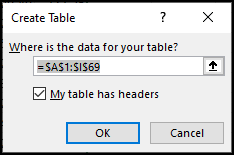
\includegraphics[width=\maxwidth{.50\linewidth}]{gfx/ch09_fig10}
		\caption{Creating a Data Table}
		\label{09:fig10}
	\end{figure}
	
	\item Click \fmtButton{OK}.
\end{enumerate}

Excel creates a data table (Figure \ref{09:fig11}), which has many of the properties expected of a database. 

\begin{figure}[H]
	\centering
	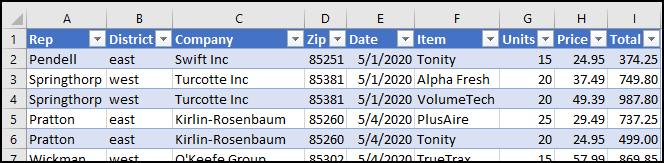
\includegraphics[width=\maxwidth{.95\linewidth}]{gfx/ch09_fig11}
	\caption{Top Of the Data Table}
	\label{09:fig11}
\end{figure}

\begin{enumerate}[resume]
	\item At \fmtButton{Table Tools $ \Rightarrow $ Properties $ \Rightarrow $ Table Name} enter \fmtTyping{Sales} as the new table name in a text box near the left edge of the ribbon.
\end{enumerate}

In a database, columns are referred to as ``Fields'' and rows as ``Records.'' Notice that each of the fields in the data table includes a drop-down arrow. That opens a menu with filtering functions that can be applied to the database. Figure \ref{09:fig12} illustrates the filter for the \textit{Item} field.

\begin{figure}[H]
	\centering
	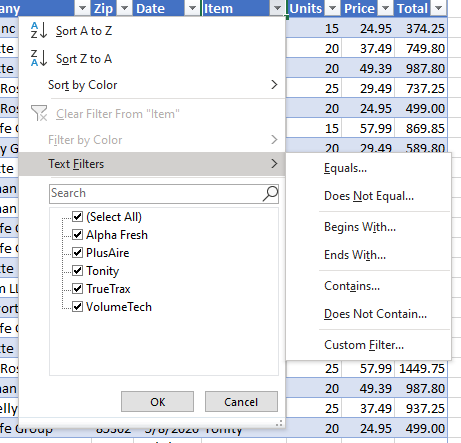
\includegraphics[width=\maxwidth{.95\linewidth}]{gfx/ch09_fig12}
	\caption{Item Filter}
	\label{09:fig12}
\end{figure}

The database can be sorted on the item field by clicking either of the top two buttons in the filter drop-down (named ``Sort A to Z'' and ``Sort Z to A''). Clicking the \textit{Text Filters} button opens a submenu where powerful filters can be created. (Note, the \textit{Filters} button for fields with other types of data, like numbers or dates, will match the data type.) Also, the checkboxes at the bottom of the popup can be used to hide or view records that match the selected item. Thus, to only see the ``Alpha Fresh'' records, uncheck all boxes except that one.

\subsection{The Database Functions}

Along with simple sorting and filtering, Excel provides the following functions that are designed to be used with a database. 

\begin{itemize}
	\item \textbf{DAVERAGE}. Calculates the average of values in a field that meet specified conditions.
	\item \textbf{DCOUNT}. Returns the number of cells containing numbers in a field that meet specified conditions.
	\item \textbf{DCOUNTA}. Returns the number of non-blank cells in a field that meet specified conditions.
	\item \textbf{DGET}. Returns a single value from a field that meet specified conditions.
	\item \textbf{DMAX}. Returns the maximum value from a field that meet specified conditions.
	\item \textbf{DMIN}. Returns the minimum value from a field that meet specified conditions.
	\item \textbf{DPRODUCT}. Calculates the product of values in a field that meet specified conditions.
	\item \textbf{DSTDEV}. Calculates the standard deviation (based on a sample of a population) of values in a field that meet specified conditions.
	\item \textbf{DSTDEVP}. Calculates the standard deviation (based on an entire population) of values in a field that meet specified conditions.
	\item \textbf{DSUM}. Calculates the sum of values in a field that meet specified conditions.
	\item \textbf{DVAR}. Calculates the variance (based on a sample of a population) of values in a field that meet specified conditions.
	\item \textbf{DVARP}. Calculates the variance (based on an entire population) of values in a field that meet specified conditions.
\end{itemize}

These functions all use similar syntax: \textit{=FuncName(Database, Field, Criteria)}. In the function, the \textit{FuncName} is the name of the function, like \textit{DSUM}. The \textit{Database} name will be \textit{Sales} in this exercise since that is the name of the table. The \textit{Field} is one of the field names, like \textit{Rep} or \textit{District}. Finally, the \textit{Criteria} is a range that contains the factors that limit the output of the function. This is best explained with some examples.

\begin{enumerate}[resume]
	\item Set up an area where the sum of all orders sent to Zip $ 85260 $ will be calculated (see Figure \ref{09:fig21}).

	\begin{itemize}
		\item In cell \fmtLoc{K2}, enter \fmtTyping{Zip}
		\item In cell \fmtLoc{K3}, enter \fmtTyping{85260}
		\item In cell \fmtLoc{L2}, enter \fmtTyping{Sum} . 
		\item In cell \fmtLoc{L3}, enter \fmtTyping{=DSUM(Sales[\#All], ''Total'', K2:K3)}. 
	\end{itemize}

	\item Here is what the various parts of the formula in \fmtLoc{L3} mean.		

	\begin{itemize}
		\item \textbf{DSUM}. This is the \textit{Data Sum} function that totals all the specified data.
		\item \textbf{Sales[\#All]}. This instructs Excel to use the entire \textit{Sales} data table. By using this nomenclature rather than specific cell locations (like \fmtLoc{A1:I69}), the formula will continue to work even if records are later added to or removed from the table.
		\item \textbf{Total}. This is the field that contains the numbers to be summed. Notice that the field name is put in quote marks.
		\item \textbf{K2:K3}. This is the location of the criteria Excel will use to sum the sales amounts. In this case, the \textit{Zip Code} must be equal to $ 85260 $.
	\end{itemize}	

	\begin{figure}[H]
		\centering
		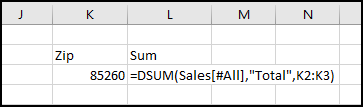
\includegraphics[width=\maxwidth{.75\linewidth}]{gfx/ch09_fig21}
		\caption{Setting Up the Data File Calculation}
		\label{09:fig21}
	\end{figure}

	\item Once the formula and criteria are entered, Excel calculates the total value of sales to that \textit{Zip Code} and displays $ 14747.55 $.
	\item Change the \textit{Zip Code} in \fmtLoc{K3} to \fmtTyping{85251}. The value in cell \fmtLoc{L3} will be automatically updated to $ 748.50 $, which is the total value in sales to that \textit{Zip Code}.
	\item Copy/paste cells \fmtLoc{K2:L3} to \fmtLoc{K5:L6}. When pasted, Excel will automatically update the criteria range in the formula to \fmtLoc{K5:K6}.
	\item Change the value of \fmtLoc{K5} to \fmtTyping{District} and \fmtLoc{K6} to \fmtTyping{east}. \fmtLoc{L6} now displays $ 22546.95 $, which is the total value of sales to the \textit{east} district.
	\item Copy/paste \fmtLoc{K5:L6} to \fmtLoc{K8:L9}.
	\item Change the formula in \fmtLoc{L9} to calculate the average value of the total sales by changing \fmtTyping{DSUM} to \fmtTyping{DAVERAGE}. The formula in \fmtLoc{L9} should now be: \fmtTyping{=DAVERAGE(Sales[\#All], ''Total'', K8:K9)}
	\item Change \fmtLoc{K8} to \fmtTyping{Rep} and \fmtLoc{K9} to \fmtTyping{Pratton}. \fmtLoc{L9} should now display $ 736.7236842 $, which is the average sale value for \textit{Pratton}. The average sale for other sellers can be easily checked by entering their names in \fmtLoc{K9}, one at a time.
	\item Save the \fmtWorksheet{CH9-Sales} workbook.
\end{enumerate}

One important feature for any database lookup is the ability to specify ``Boolean'' matches; that is, a match that includes an AND term or an OR term. For example, that would answer a question like, ``What is the total value of the sales of TrueTrax made by Findlay?'' Follow these steps to create Boolean expressions.

\begin{enumerate}
	\item Copy/paste \fmtLoc{K8:K9} to \fmtLoc{K11:K12} and paste \fmtLoc{K8:K9} to \fmtLoc{L11:L12}. Be sure \fmtLoc{K11} is \fmtTyping{Rep}, then change \fmtLoc{K12} to \fmtTyping{Findlay}, \fmtLoc{L11} to \fmtTyping{Item} and \fmtLoc{L12} to \fmtTyping{TrueTrax}.
	\item Copy/paste \fmtLoc{L8:L9} to \fmtLoc{M11:M12}. Change the formula in \fmtLoc{M12} to \fmtTyping{=DSUM(Sales[\#All], ''Total'', K11:L12)}. 
	
	\begin{figure}[H]
		\centering
		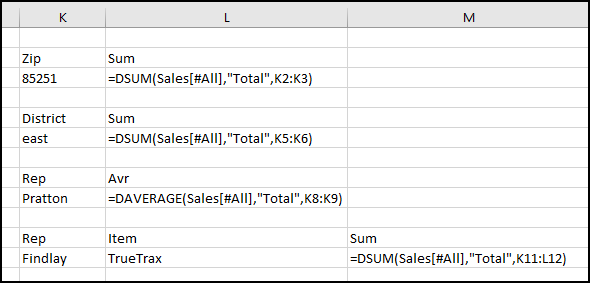
\includegraphics[width=\maxwidth{.95\linewidth}]{gfx/ch09_fig22}
		\caption{Calculating an AND Expression}
		\label{09:fig22}
	\end{figure}
	
	\item Cell \fmtLoc{M12} is now $ 1739.7 $, which is the total value of Findlay's \textit{TrueTrax} sales. Note, if the value in \fmtLoc{M12} is not right, check for typos in the \textit{Rep} and \textit{Item} names.
	\item Data criteria items that appear in the same row are combined with an AND, so the range \fmtLoc{K11:L12} would be read ``Calculate the sum of all lines that include a representative named Findlay AND an item named TrueTrax.''
	\item Note: The order of the ANDed terms is important. They must be in the same order in the criteria section as they are in the data table. Therefore, if \textit{Item} were in \fmtLoc{K11} and \textit{Rep} in \fmtLoc{L11} the formula would fail since these two variables are in the opposite order as the data fields in the table.
	\item Other sales representative names can be entered in cell \fmtLoc{K12} or other items in \fmtLoc{L12} to check on those sales.
	\item To combine two or more terms with an OR, place those terms on separate lines, as demonstrated next.
	\item Copy/paste \fmtLoc{K11:M12} to \fmtLoc{K14:M15}.
	\item Rather than calculate the total value of \textit{Findlay's} sales, count the number of items sold. Change \fmtLoc{M14} to \fmtTyping{Units Sold}.
	\item Change the formula in \fmtLoc{M15} to: \fmtTyping{=DSUM(Sales[\#All], ''Units'', K14:L15)}. Notice that the only change to the formula is that it will sum the \textit{Units} field instead of the \textit{Total} field.
	\item To include \textit{PlusAir}, in cell \fmtLoc{K16}, enter \fmtTyping{Findlay} and in cell \fmtLoc{L16}, enter \fmtTyping{PlusAir}.
	\item Change the formula in \fmtLoc{M15} to \fmtTyping{=DSUM(Sales[\#All], ''Units'', K14:L16)}. Notice that the only change is to increase the criteria range to \fmtLoc{K14:L16}. Now, Excel will count the total number of lines that include both \textit{Findlay} and \textit{TrueTrax} OR \textit{Findley} and \textit{PlusAir}. Excel reports that \textit{Findlay} sold $ 50 $ \textit{TrueTrax} OR \textit{PlusAir} units.
	
	\begin{figure}[H]
		\centering
		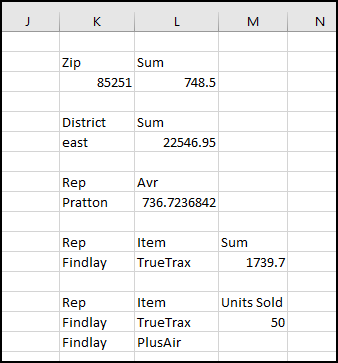
\includegraphics[width=\maxwidth{.75\linewidth}]{gfx/ch09_fig23}
		\caption{Calculating an OR Expression}
		\label{09:fig23}
	\end{figure}
\end{enumerate}

Finally, it is often desirable to set up a range for a data calculation. For example, it is possible to count the total number of \textit{Tonity} sales made between May $ 5 $ and May $ 20 $.

\begin{enumerate}
	\item In both cells \fmtLoc{K18} and \fmtLoc{L18}, enter \fmtTyping{Date} (the \textit{Date} will be entered two times in the criteria); in cell \fmtLoc{M18}, enter \fmtTyping{Item}; and in cell \fmtLoc{N18}, enter \fmtTyping{Count}.
	\item In cell \fmtLoc{K19}, enter \fmtTyping{$>$=5/10/2020}; in cell \fmtLoc{L19}, enter \fmtTyping{$<$=5/20/2020}; and in cell \fmtLoc{M19}, enter \fmtTyping{Tonity}.
	\item In cell \fmtLoc{N19}, enter  \fmtTyping{=DCOUNT(Sales[\#All], ''Total'', K18:M19)}. Notice that this is a \textit{DCOUNT} formula, so the number of lines that contain a \textit{Tonity} item sold between $ 5/10/2020 $ and $ 5/20/2020 $ (inclusive) will be counted.
	
	\begin{figure}[H]
		\centering
		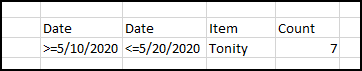
\includegraphics[width=\maxwidth{.95\linewidth}]{gfx/ch09_fig24}
		\caption{Specifying a Date Range}
		\label{09:fig24}
	\end{figure}

	\item Excel reports seven \textit{Tonity} sales were made between the two specified dates.
	\item Save and close the \fmtWorksheet{CH9-Sales} workbook.

\end{enumerate}

Creating a data table is easy in Excel, then the \textit{Data} formulas make it easy to create complex calculations by simply specifying the desired criteria in a range of cells.
	
\begin{center}
	\begin{tkwbox}{Key Take-Aways}
		\textbf{Database Functions}
		\\
		\begin{itemize}
			\setlength{\itemsep}{0pt}
			\setlength{\parskip}{0pt}
			\setlength{\parsep}{0pt}
			
			\item Set up the database functions by creating a data table.
			\item Use any of the ``D...'' functions to easily count, sum, or statistically analyze a data table using complex Boolean operations. 
			
		\end{itemize}
	\end{tkwbox}
\end{center}

\section{Useful Functions}

\begin{center}
	\begin{objbox}{Learning Objectives}
		\begin{itemize}
			\setlength{\itemsep}{0pt}
			\setlength{\parskip}{0pt}
			\setlength{\parsep}{0pt}
			
			\item Practice with $ 8 $ of Excel's most useful text functions.
			\item Practice with $ 12 $ of Excel's most useful numeric functions.
			
		\end{itemize}
	\end{objbox}
\end{center}

Excel includes more than $ 300 $ functions that are designed to process both text and numbers. Most of those functions are only useful in specific situations and most users will never know that they exist; however, many functions are so commonly used that they show up in many spreadsheet projects. This section provides information and practice with $ 20 $ of the most useful Excel functions.

A contact roster will be used for the exercises in this section. This file contains information that would be used by sales representatives as they work with a company's clients. The roster needs to be cleaned up a bit for more efficient use. (Note: this roster contains fake data.)

\begin{enumerate}
	\item Open workbook \fmtWorksheet{CH9-ContactData.xlsx}
	\item Save the workbook as \fmtWorksheet{CH9-Contact.xlsx}.
	\item This workbook has only one worksheet, \fmtWorksheet{Contacts}.
\end{enumerate}

\subsection{Text Functions}

Excel includes scores of functions designed to be used with cells that contain text rather than numbers and this section explores the most used text functions.

\subsubsection{To Columns}

Often, a field in a data file contains two or more separate pieces of information. This makes it impossible to complete tasks like sorting on the individual pieces of information. The \textit{Name} data field (\textit{Column B}) in the \textit{Contacts} worksheet includes both first and last names, but those should be placed in different fields. This is such a common operation; Excel has a function that splits data separated by a comma into two different fields.

\begin{enumerate}
	\item Insert a new column to the left of \fmtLoc{Column C}. This column will eventually contain the first name and \fmtLoc{Column B} will contain the last name.
	\item Click \fmtLoc{B2} and then shift-click \fmtLoc{B101} to select all the data in \fmtLoc{Column B}. (Note: a useful keyboard shortcut is to click \fmtLoc{B2} then \fmtKeystroke{Ctrl} + \fmtKeystroke{Shift} + \fmtKeystroke{Down Arrow} to select all data in the column.)
	\item Click \fmtButton{Data $ \Rightarrow $ Data Tools $ \Rightarrow $ Text to Columns}.
	\item Excel starts a data wizard to help split the data. The first screen is used to adjust from delimited to fixed width data type, but the default, delimited, is correct, so click \fmtButton{Next}.
	
	\begin{figure}[H]
		\centering
		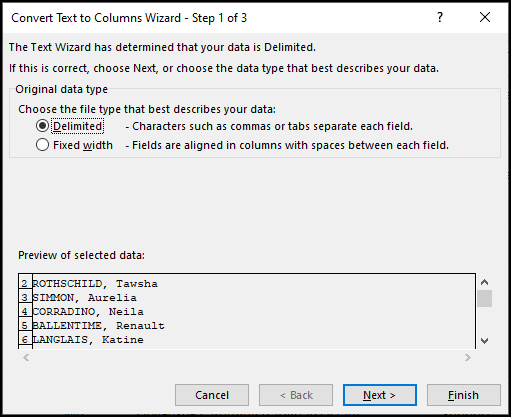
\includegraphics[width=\maxwidth{.75\linewidth}]{gfx/ch09_fig30}
		\caption{Convert Text to Columns Wizard Screen 1}
		\label{09:fig30}
	\end{figure}

	\item The second wizard box determines what sort of delimiter is used with the data. For this field, the first and last names are separated by a comma, so check the \fmtButton{Comma} delimiter and uncheck the \fmtButton{Tab} delimiter. The sample data at the bottom of the Wizard screen should show the first and last names divided. Click \fmtButton{Next}.

	\begin{figure}[H]
		\centering
		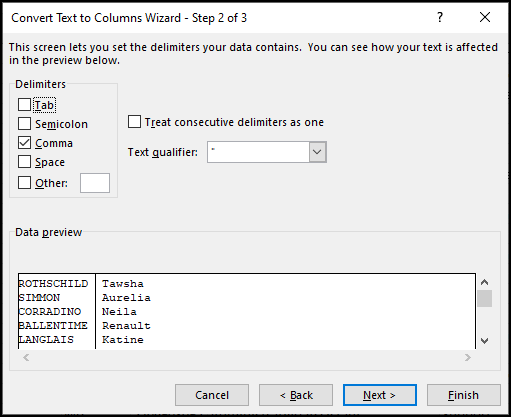
\includegraphics[width=\maxwidth{.75\linewidth}]{gfx/ch09_fig31}
		\caption{Convert Text to Columns Wizard Screen 2}
		\label{09:fig31}
	\end{figure}

	\item The third wizard box determines the type of data each column contains. Since the default, \textit{General}, is appropriate, click \fmtButton{Finish}.

	\begin{figure}[H]
		\centering
		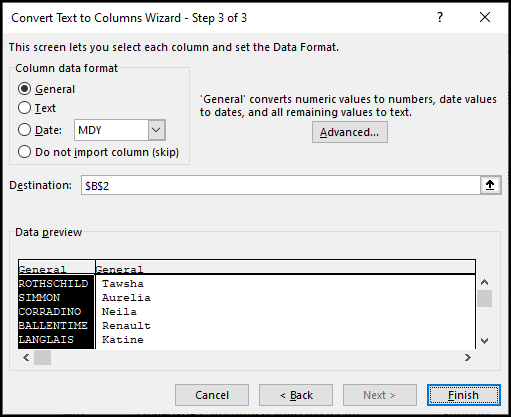
\includegraphics[width=\maxwidth{.75\linewidth}]{gfx/ch09_fig32}
		\caption{Convert Text to Columns Wizard Screen 3}
		\label{09:fig32}
	\end{figure}

	\item Excel splits the names into two columns. 
	\item In cell \fmtLoc{B1} enter \fmtTyping{Last\_Name} (with an underscore).
	\item In cell \fmtLoc{C1} enter \fmtTyping{First\_Name} (with an underscore).
	\item Adjust \fmtLoc{Column B} and \fmtLoc{Column C} so they are the optimum width.
	
	\begin{figure}[H]
		\centering
		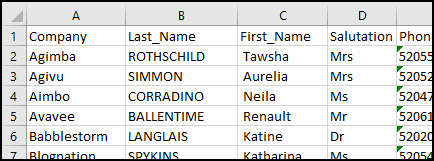
\includegraphics[width=\maxwidth{.95\linewidth}]{gfx/ch09_fig33}
		\caption{Names Divided Into Two Columns}
		\label{09:fig33}
	\end{figure}
\end{enumerate}

\subsubsection{Trim}

\[ =TRIM(text) \]

The TRIM function is used to trim unwanted spaces from the start or end of text in a cell.

\begin{enumerate}
	\item This exercise uses the \fmtWorksheet{Contacts} worksheet in the \fmtWorksheet{Contact} workbook.
	\item When the name was separated into \textit{Last\_Name} and \textit{First\_Name} columns, Excel automatically added a space at the start of the \textit{First\_Name} field. That space, though, will be a problem in later exercises. 
	\item Insert a new column to the left of \fmtLoc{Column D}. The newly inserted column becomes \fmtLoc{Column D}.
	\item In cell \fmtLoc{D2}, enter \fmtTyping{=TRIM(C2)}.
	\item Copy \fmtLoc{D2} to \fmtLoc{D3:D101}. This removes the leading space from the first names.
	\item Select and copy \fmtLoc{D2:D101}.
	\item Click \fmtLoc{C2} then \fmtButton{Home $ \Rightarrow $ Clipboard $ \Rightarrow $ Paste $ \Rightarrow $ Values}. Note: it is important to paste the values, not just a simple paste. Otherwise, \fmtLoc{C2:C101} will be filled with the \textit{TRIM} formula rather than the value generated by that formula.
	
	\begin{figure}[H]
		\centering
		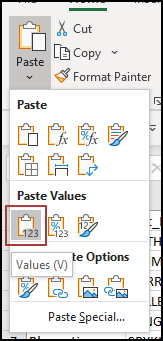
\includegraphics[width=\maxwidth{.65\linewidth}]{gfx/ch09_fig34}
		\caption{Paste Values Button}
		\label{09:fig34}
	\end{figure}
	
	\item Delete \fmtLoc{Column D}.
	\item Though it is not visible, the data in \fmtLoc{Column F} (the \textit{Role} column) has a random number of spaces trailing many of the entries, which is a common problem caused by sloppy data entry.
	\item Insert a new column to the left of \fmtLoc{Column G}. The newly inserted column becomes \fmtLoc{Column G}.
	\item In cell \fmtLoc{G2}, enter \fmtTyping{=TRIM(F2)}.
	\item Copy \fmtLoc{G2} to \fmtLoc{G3:G101}. This removes the trailing space from all entries in the role data.
	\item Select and copy \fmtLoc{G2:G101}.
	\item Click \fmtLoc{F2} then \fmtButton{Home $ \Rightarrow $ Clipboard $ \Rightarrow $ Paste $ \Rightarrow $ Values}. Note: it is important to paste the values, not just a simple paste. Otherwise, \fmtLoc{F2:F101} will be filled with the \textit{TRIM} formula rather than the value generated by that formula.
	\item Delete \fmtLoc{Column G}.
\end{enumerate}

\subsubsection{Upper/Lower/Proper}

\[ =UPPER(text) \]
\[ =LOWER(text) \]
\[ =PROPER(text) \]

Often, the text case needs to be changed. The UPPER function changes text to upper case, the LOWER function changes text to lower case, and the PROPER function changes to title case (the first letter of each word is capitalized). 

\begin{enumerate}
	\item This exercise uses the \fmtWorksheet{Contacts} worksheet in the \fmtWorksheet{Contact} workbook.
	\item For some reason, the last names in \fmtLoc{Column B} are uppercase. Uppercase text is commonly found, but that type of text is difficult to read.
	\item Insert a new column to the left of \fmtLoc{Column C}. The newly inserted column becomes \fmtLoc{Column C}.
	\item Enter this formula in \fmtLoc{C2}: \fmtTyping{=PROPER(B2)}.
	\item Copy \fmtLoc{C2} to \fmtLoc{C3:C101}. This changes the last names to proper case.
	\item Select and copy \fmtLoc{C2:C101}.
	\item Click \fmtLoc{B2} then \fmtButton{Home $ \Rightarrow $ Clipboard $ \Rightarrow $ Paste $ \Rightarrow $ Values}. Note: it is important to paste the values, not just a simple paste. Otherwise, \fmtLoc{B2:B101} will be filled with the \textit{PROPER} formula rather than the value generated by that formula.
	\item Delete \fmtLoc{Column C}.
\end{enumerate}

\subsubsection{Left/Right/Mid}

\[ =LEFT(text, [num\_chars]) \]
\[ =RIGHT(text, [num\_chars]) \]
\[ =MID(text, start\_num, [num\_chars]) \]

The LEFT, RIGHT, and MID functions are used to extract letters from a text field. For example, cell \textit{B2} contains \textit{Rothschild}. The function \textit{=LEFT(B2,4)} would extract ``Roth,'' the left four letters in that field. The function \textit{=RIGHT(B2,5)} would extract ``child,'' the right five letters in that field. The function \textit{=MID(B2,5,3)} would extract ``sch,'' the three letters starting in position five in that field. These functions, along with CONCATENATE in the next section, are used to change the format of the phone number (\textit{Column E}) from ten digits to (xxx) xxx-xxxx.

\subsubsection{Concatenate}

\[ =CONCATENATE(text1, text2, [text3], ...) \]

Frequently, text stored in various workbook cells needs to be combined to create new information. The CONCATENATE function makes this possible. The various text phrases to combine are entered one after another, separated by commas. This exercise uses CONCATENATE along with LEFT, RIGHT, and MID to change the format of the phone number in \textit{Column E} from ten digits to (xxx) xxx-xxxx.

\fmtNewExcel{Excel 365} Note: this function was renamed \textit{CONCAT} in Excel $ 365 $.

\begin{enumerate}
	\item This exercise uses the \fmtWorksheet{Contacts} worksheet in the \fmtWorksheet{Contact} workbook.
	\item Insert a new column to the left of \fmtLoc{Column F}. The newly inserted column becomes \fmtLoc{Column F}.
	\item Enter this in \fmtLoc{F2}: \fmtTyping{=CONCATENATE("(", LEFT(E2,3),") ",\\MID(E2,4,3), "-", RIGHT(E2,4))}
	\item The formula concatenates (or joins) an open parenthesis, the left three digits of the phone number, a closing parenthesis with a space, the three middle digits of the phone number, a dash, and the right four digits of the phone number. The formula looks complex but is easy to understand if it is built up one small piece at a time.
	\item Copy \fmtLoc{F2} to \fmtLoc{F3:F101}. This changes the format of the phone number to (xxx) xxx-xxxx.
	\item Select and copy \fmtLoc{F2:F101}.
	\item Click \fmtLoc{E2} then \fmtButton{Home $ \Rightarrow $ Clipboard $ \Rightarrow $ Paste $ \Rightarrow $ Values}. Note: it is important to paste the values, not just a simple paste. Otherwise, \fmtLoc{E2:E101} will be filled with the \textit{CONCATENATE} formula rather than the value generated by that formula.
	\item Delete \fmtLoc{Column F}.
	\item Adjust the width of \fmtLoc{Column E} to properly display the formatted phone number.
	\item Save the \fmtWorksheet{CH9-Contact} workbook.
\end{enumerate}

\subsubsection{Search}	

\[ =SEARCH(find\_text, within\_text, [start\_num]) \]

The SEARCH function is used to find a phrase in a cell that contains text. This is like the LEFT/RIGHT/MID functions except with SEARCH the exact starting position of the target data is not known in advance. Therefore, SEARCH could be used to find the phrase ``good'' in strings like ``good morning'' and ``the greater good'' where the target phrase starts in different locations in each string. Optionally, a start point for the search can be specified. SEARCH returns the position where the target phrase starts, so SEARCH would report that ``good'' in ``good morning'' starts at position one but in ``the greater good'' it starts at position $ 13 $. For this exercise, the year needs to be extracted from the \textit{Contract\_Num} field (\textit{Column J}). The starting position for the year varies but is always after the first dash (see Figure \ref{09:fig35}), so SEARCH is needed instead of a simple LEFT/RIGHT/MID function. Note: SEARCH is not case sensitive, but the related Excel function FIND is case sensitive. Other than that, the two functions are identical. Thus, to locate the word ``College'' in a cell, use SEARCH if the capital letter should be ignored but FIND if the capital letter is important.

\begin{enumerate}
	\item This exercise uses the \fmtWorksheet{Contacts} worksheet in the \fmtWorksheet{Contact} workbook.
	\item Insert a new column to the left of \fmtLoc{Column K}. The newly inserted column becomes \fmtLoc{Column K}.
	\item In cell \fmtLoc{K1}, enter \fmtTyping{Year}. This column will contain the extracted year.
	\item In cell \fmtLoc{K2}, enter \fmtTyping{=VALUE(MID(J2, SEARCH("-", J2)+1,4))}. If the formula is entered without error, cell \fmtLoc{K2} will display $ 2013 $, the year in the contract number in cell \fmtLoc{J2}. This is a complex formula, but it can be broken down, starting in the middle of the formula: 
	
	\begin{itemize}
		\item \textbf{SEARCH(``-'',J2)}. Search for a hyphen in data field \fmtLoc{J2}.
		\item \textbf{MID(J2, SEARCH("-", J2)+1,4)}. Using the MID function, extract from data field \fmtLoc{J2}, starting one letter past the position of the hyphen, for four characters.
		\item \textbf{=VALUE(MID(J2, SEARCH("-", J2)+1,4))}. Convert the extracted text to a number rather than store it as text. Note: Excel would store an extracted phrase as text, but since these are years it is sensible to store them as numbers so various statistical functions can later be used.
	\end{itemize}

	\item Copy \fmtLoc{K2} to \fmtLoc{K3:K101}. This finds the year from each of the contract numbers.
	\item Select and copy \fmtLoc{K2:K101}.
	\item Click \fmtLoc{K2} then \fmtButton{Home $ \Rightarrow $ Clipboard $ \Rightarrow $ Paste $ \Rightarrow $ Values}. Note: This looks odd since the cells are being pasted back into the same locations from which they were copied, but this is a good way to remove a formula from a cell without creating an additional data column. It is important to paste the values, not just a simple paste. Otherwise, \fmtLoc{K2:K101} will be filled with the \textit{SEARCH} formula rather than the value generated by that formula.
	\item Adjust the width of \fmtLoc{Column K} to optimally fit the year data.
	
	\begin{figure}[H]
		\centering
		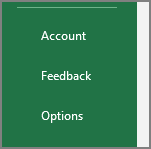
\includegraphics[width=\maxwidth{.65\linewidth}]{gfx/ch09_fig35}
		\caption{Extracting the Year from the Contract Number}
		\label{09:fig35}
	\end{figure}
	
\end{enumerate}

\subsubsection{VLookup}

\[ =VLOOKUP(value, table, col\_index, [approx]) \]

VLOOKUP is a useful, but complex, Excel function. It is used to look up and return a value from a table. VLOOKUP will look up some target value in column one of a data range and return the value from an indexed column number. This concept is much easier to understand with an example. Consider Table \ref{09:tab01}.

\begin{table}[H]
	\rowcolors{1}{}{tablerow} % zebra striping background
	{\small
		%\fontsize{8}{10} \selectfont %Replace small for special font size
		\begin{longtable}{L{0.30in}L{0.50in}L{1.00in}L{0.50in}} %Left-aligned, Max width: 4.25in
			\textbf{ID} & \textbf{Name} & \textbf{Phone} & \textbf{Section} \endhead
			\hline
			0134 & Jones & (520) 123-4567 & Sales\\
			0293 & Marks & (520) 398-2219 & HR\\
			0342 & Nash  & (520) 721-9043 & Orders\\
			\rowcolor{captionwhite}
			\caption{VLookup Example Table}
			\label{09:tab01}
		\end{longtable}
	} % End small
\end{table}

The formula \textit{=VLOOKUP(0293,A2:D5,4)} would lookup \textit{0293} in the first column of the data table in \textit{A2:D5} and then return the value in the fourth column of that table, \textit{HR}.

The last parameter in the VLOOKUP function, ``approx,'' determines if the match in column can be approximate or if an exact match is required. If the value for this item is TRUE then an approximate match is acceptable (this is the default), but if it is FALSE then the match must be exact. 

\begin{enumerate}
	\item This exercise uses the \fmtWorksheet{Contacts} worksheet in the \fmtWorksheet{Contact} workbook.
	\item In cell \fmtLoc{P3} enter \fmtTyping{Company}.
	\item In cell \fmtLoc{P4} enter \fmtTyping{Last Name}.
	\item In cell \fmtLoc{P5} enter \fmtTyping{Phone}.
	\item In cell \fmtLoc{P6} enter \fmtTyping{Role}.
	\item Adjust the width of \fmtLoc{Column P} to optimally fit the data.
	\item In cell \fmtLoc{Q3} enter \fmtTyping{Agimba}. This is the name of the first company, found in cell \fmtLoc{A2}.
	\item In cell \fmtLoc{Q4} enter \fmtTyping{=VLOOKUP(\$Q\$3,\$A\$1:\$F\$101,2,FALSE)}. This formula will lookup the company found in cell \fmtLoc{Q3}, ``Agimba,'' in column one of the table found in \fmtLoc{A1:F101} and then return the value found in column two of that table (see Figure \ref{09:fig36}). When completed, cell \fmtLoc{Q4} should contain \textit{Rothschild}, which is the name of the representative at \textit{Agimba}. If the cell contains an error message check the formula for typing errors and check the spelling of \textit{Agimba} in cell \fmtLoc{Q3}. Notice that the formula uses absolute references so if it is copied to other cells it will still refer to the correct table. Also notice that the last item in the formula is ``FALSE'' which makes Excel look for an exact match rather than an approximate match.
	\item In cell \fmtLoc{Q5} enter \fmtTyping{=VLOOKUP(\$Q\$3,\$A\$1:\$F\$101,5,FALSE)}. This is the same formula entered in \textit{Q4}, but the column returned is $ 5 $ instead of $ 2 $. This formula will lookup the company found in cell \fmtLoc{Q3}, ``Agimba,'' in column one of the table found in \fmtLoc{A2:F101} and then return the value found in column five of that table. When completed, cell \fmtLoc{Q5} should contain ``(520) 555-1082,'' which is Agimba's phone number.  Notice that the formula uses absolute references so if it is copied to other cells it will still refer to the correct table. Also notice that the last item is ``FALSE'' which makes Excel look for an exact match rather than an approximate match.
	\item In cell \fmtLoc{Q6} enter \fmtTyping{=VLOOKUP(\$Q\$3, \$A\$1:\$F\$101, 6, FALSE)}. This is the same formula entered in \textit{Q5}, but the column returned is $ 6 $ instead of $ 5 $. This formula will lookup the company found in cell \fmtLoc{Q3}, ``Agimba,'' in column one of the table found in \fmtLoc{A2:F101} and then return the value found in column six of that table. When completed, cell \fmtLoc{Q6} should contain ``Business Analyst,'' which is the role of the contact at Agimba.  Notice that the formula uses absolute references so if it is copied to other cells it will still refer to the correct table. Also notice that the last item is ``FALSE'' which makes Excel look for an exact match rather than an approximate match.
	
	\begin{figure}[H]
		\centering
		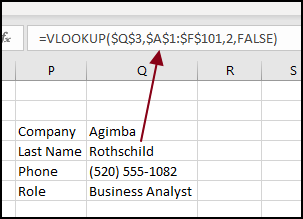
\includegraphics[width=\maxwidth{.75\linewidth}]{gfx/ch09_fig36}
		\caption{VLookup Formula for Q4}
		\label{09:fig36}
	\end{figure}
	
	\item Adjust the width of \fmtLoc{Column Q} to optimally fit the data.
	\item If the company in cell \fmtLoc{Q3} is changed then the data displayed in \fmtLoc{Q4:Q6} will be updated to match the new name. Try entering \fmtTyping{Blogtag} and \fmtTyping{Eidel} in \fmtLoc{Q3} to check the update feature.
\end{enumerate}

\subsubsection{Index Match}

\[ =INDEX(data,MATCH(value,lookup\_column,FALSE),column) \]

This is the most complex formula in this book and is a combination of two simpler functions: INDEX and MATCH. On the surface, it does almost exactly what VLOOKUP does, so many people do not bother to learn the INDEX MATCH formula. However, VLOOKUP requires the lookup field to be in column one of the data table while INDEX MATCH can look up data in any column. Also, if the data table is changed in some way (a new column added, for example), VLOOKUP will no longer work but INDEX MATCH will adapt to the new table structure. So, the time taken to learn this lookup formula will result in a more robust lookup function.

\begin{enumerate}
	\item This exercise uses the \fmtWorksheet{Contacts} worksheet in the \fmtWorksheet{Contact} workbook.
	\item In cell \fmtLoc{P8} enter \fmtTyping{Contract Num}.
	\item In cell \fmtLoc{P9} enter \fmtTyping{Company}.
	\item In cell \fmtLoc{P10} enter \fmtTyping{Phone}.
	\item In cell \fmtLoc{P11} enter \fmtTyping{Last Name}.
	\item Adjust the width of \fmtLoc{Column P} to optimally fit the data.
	\item In cell \fmtLoc{Q8} enter \fmtTyping{Agim(BusDev)-2013-21}. This is the contract number for the first data row, found in cell \fmtLoc{J2}.
	\item In cell \fmtLoc{Q9} enter \fmtTyping{=INDEX(\$A\$2:\$F\$101, MATCH(\$Q\$8, \\\$J\$2:\$J\$101, FALSE), 1)} (see Figure \ref{09:fig37}). (Note: if \textit{Q9} displays an error then check the formula in \fmtLoc{Q9} and the value in \fmtLoc{Q8} for typing errors.) This is a complex formula and it will help to break it down into smaller chunks, starting in the middle: 
	
	\begin{itemize}
		\item \textbf{MATCH(\$Q\$8,\$J\$2:\$J\$101,FALSE)}. In the center of the complex formula is a \textit{MATCH} function. That will look for the value in cell \fmtLoc{Q8} (the contract number) in \fmtLoc{J2:J101} (the contract data field). An exact match is required since the last parameter is FALSE. If the contract number is found, then MATCH will return the row number for that contract.
		\item \textbf{=INDEX(\$A\$2:\$F\$101,RowNum,1)}. \textit{INDEX} will use the row number (\textit{RowNum}) returned by the \textit{MATCH} function and return the data in column one (Company name) of the data table in \fmtLoc{A2:F101}.
	\end{itemize}
		
	\item When completed, cell \fmtLoc{Q9} should contain ``Agimba,'' which is the name of the company for the contract number in cell \fmtLoc{Q8}. Notice that the formula uses absolute references so if it is copied to other cells it will still refer to the correct table.
	\item In cell \fmtLoc{Q10} enter \fmtTyping{=INDEX(\$A\$2:\$F\$101, MATCH(\$Q\$8, \\\$J\$2:\$J\$101,FALSE),5)}. This is the same formula entered in \textit{Q9}, but the last number is changed from $ 1 $ to $ 5 $ to return the phone number field. This formula will match the contract number found in cell \fmtLoc{Q8} and then return the value found in column five of the data table. When completed, cell \fmtLoc{Q10} should contain ``(520) 555-1082,'' which is the phone number for the company.  Notice that the formula uses absolute references so if it is copied to other cells it will still refer to the correct table. 
	\item In cell \fmtLoc{Q11} enter \fmtTyping{=INDEX(\$A\$2:\$F\$101, MATCH(\$Q\$8, \\\$J\$2:\$J\$101,FALSE),2)}. This is the same formula entered in \textit{Q10}, but the last number is changed from $ 5 $ to $ 2 $ to return the last name field. This formula will look up the contract number found in cell \fmtLoc{Q8} and then return the value found in column two of the data table. When completed, cell \fmtLoc{Q11} should contain ``Rothschild,'' which is the last name of the contact for this contract.  Notice that the formula uses absolute references so if it is copied to other cells it will still refer to the correct table. 
	
	\begin{figure}[H]
		\centering
		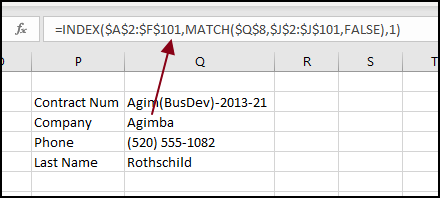
\includegraphics[width=\maxwidth{.95\linewidth}]{gfx/ch09_fig37}
		\caption{Index-Match Formula for Q9}
		\label{09:fig37}
	\end{figure}
	
	\item If the contract number in \fmtLoc{Q8} is changed then the data displayed in \fmtLoc{Q9:Q11} will be updated to match the new number. Try entering \fmtTyping{Buzz(Sales)-2014-117} and \fmtTyping{Link(RD)-2013-21} in \fmtLoc{Q8} to check the update feature.
	\item Save the \fmtWorksheet{CH9-Contact} workbook.
		
\end{enumerate}

\subsection{Number Functions}

Excel has hundreds of functions designed to be used with cells that contain numbers and this section explores the most used number functions.

\subsubsection{Sum}

\[ =SUM(number1, [number2], [number3], ...) \]

This function adds all the values in a specified range. 

\begin{enumerate}
	\item This exercise uses the \fmtWorksheet{Contacts} worksheet in the \fmtWorksheet{Contact} workbook.
	\item In cell \fmtLoc{P13}, enter \fmtTyping{Total Value}.
	\item In cell \fmtLoc{Q13}, enter \fmtTyping{=SUM(L2:L101)}. This formula will total all the contract values found in \fmtLoc{Column L}.
	\item When completed, cell \fmtLoc{Q13} should contain $ 4374391 $. This number could be formatted with Excel's formatting tools to be easier to read.

	\begin{figure}[H]
		\centering
		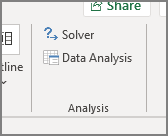
\includegraphics[width=\maxwidth{.75\linewidth}]{gfx/ch09_fig38}
		\caption{Sum Formula for Q13}
		\label{09:fig38}
	\end{figure}
	
\end{enumerate}

\subsubsection{Average}

\[ =AVERAGE(number1, [number2], [number3], ...) \]

This function calculates the average for the values in a specified range. 

\begin{enumerate}
	\item This exercise uses the \fmtWorksheet{Contacts} worksheet in the \fmtWorksheet{Contact} workbook.
	\item In cell \fmtLoc{P14}, enter \fmtTyping{Average Value}.
	\item In cell \fmtLoc{Q14}, enter \fmtTyping{=AVERAGE(L2:L101)}. This formula will calculate the average of the contract values found in \fmtLoc{Column L}.
	\item When completed, cell \fmtLoc{Q14} should contain $ 43743.91 $. This number could be formatted with Excel's formatting tools to be easier to read.

	\begin{figure}[H]
		\centering
		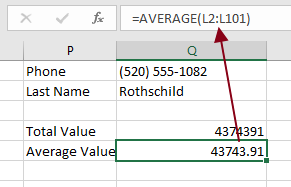
\includegraphics[width=\maxwidth{.75\linewidth}]{gfx/ch09_fig39}
		\caption{Average Formula for Q14}
		\label{09:fig39}
	\end{figure}

\end{enumerate}

\subsubsection{Min/Max}

\[ =MIN(number1, [number2], [number3], ...) \]
\[ =MAX(number1, [number2], [number3], ...) \]

These functions find the minimum or maximum value in a specified range. 

\begin{enumerate}
	\item This exercise uses the \fmtWorksheet{Contacts} worksheet in the \fmtWorksheet{Contact} workbook.
	\item In cell \fmtLoc{P15}, enter \fmtTyping{Max Value}.
	\item In cell \fmtLoc{Q15}, enter \fmtTyping{=MAX(L2:L101)}. This formula will find the maximum contract value in \fmtLoc{Column L}.
	\item When completed, cell \fmtLoc{Q15} should contain $ 88050 $.
	\item In cell \fmtLoc{P16}, enter \fmtTyping{Min Value}.
	\item In cell \fmtLoc{Q16}, enter \fmtTyping{=MIN(L2:L101)}. This formula will find the minimum contract value in \fmtLoc{Column L}.
	\item When completed, cell \fmtLoc{Q16} should contain $ 5140 $.

	\begin{figure}[H]
		\centering
		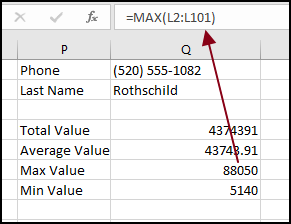
\includegraphics[width=\maxwidth{.75\linewidth}]{gfx/ch09_fig40}
		\caption{Max Formula for Q15}
		\label{09:fig40}
	\end{figure}

\end{enumerate}

\subsubsection{Round}

\[ =ROUND(number, num\_digits) \]

This function rounds a number to a specified number of digits. If the number of digits is a positive number, then it will be rounded to a decimal value but if the number of digits is negative then it will be rounded to the nearest multiple of ten. Table \ref{09:tab02} will help to clarify this concept.

\begin{table}[H]
	\rowcolors{1}{}{tablerow} % zebra striping background
	{\small
		%\fontsize{8}{10} \selectfont %Replace small for special font size
		\begin{longtable}{R{0.75in}C{0.80in}R{0.60in}L{1.50in}} %Left-aligned, Max width: 4.25in
			\textbf{Number} & \textbf{Num\_Digits} & \textbf{Result} & Notes \endhead
			\hline
			5678.1234 &  3 & 5678.123 & 3 decimal places \\
			5678.1234 &  2 & 5678.12  & 2 decimal places\\
			5678.1234 &  1 & 5678.1   & 1 decimal place\\
			5678.1234 &  0 & 5678     & Nearest whole number\\
			5678.1234 & -1 & 568      & Nearest 10\\
			5678.1234 & -2 & 57       & Nearest 100\\
			5678.1234 & -3 & 6        & Nearest 1,000\\
			\rowcolor{captionwhite}
			\caption{Rounding Places}
			\label{09:tab02}
		\end{longtable}
	} % End small
\end{table}

\begin{enumerate}
	\item This exercise uses the \fmtWorksheet{Contacts} worksheet in the \fmtWorksheet{Contact} workbook.
	\item In cell \fmtLoc{P18}, enter \fmtTyping{Rounded Value}.
	\item In cell \fmtLoc{Q18}, enter \fmtTyping{=ROUND(Q13,-4)}. This formula will round the \textit{Total Value} in cell \fmtLoc{Q13} to the nearest $ 10,000 $.
	\item When completed, cell \fmtLoc{Q18} should contain $ 4370000 $. This number could be formatted with Excel's formatting tools to be easier to read.
	\item Save the \fmtWorksheet{CH9-Contact} workbook.
\end{enumerate}

\subsubsection{If}

\[ =IF(logical\_test, [value\_if\_true], [value\_if\_false]) \]

The IF function fills a cell with some value based on the result of an ``if'' decision. As an example of the IF function, a cell on the \textit{Contacts} worksheet will be used to indicate if the value of a contract is greater than a specified threshold.

\begin{enumerate}
	\item This exercise uses the \fmtWorksheet{Contacts} worksheet in the \fmtWorksheet{Contact} workbook.
	\item Insert a new column to the left of \fmtLoc{Column M}. The newly inserted column becomes \fmtLoc{Column M}.
	\item In cell \fmtLoc{M1}, enter \fmtTyping{Priority}.
	\item Adjust the width of \fmtLoc{Column M} to properly display cell \fmtLoc{M1}.
	\item In cell \fmtLoc{M2}, enter \fmtTyping{=IF(L2\textgreater50000, "High", "Low")}. This formula will check the value in cell \fmtLoc{L2} and if it is greater than $ 50000 $ it will enter the word \textit{High} in \fmtLoc{M2} otherwise it will enter the word \textit{Low}.
	\item When completed, cell \fmtLoc{M2} should contain \textit{Low}.
	\item Copy cell \fmtLoc{M2} to \fmtLoc{M3:M10}. Notice that if the value in \fmtLoc{Column L} is greater than $ 50000 $ then \fmtLoc{Column M} will display \textit{High}, otherwise it will display the word \textit{Low}.
	\item Commonly, \textit{IF} functions are nested to get a more granular output. For this worksheet, to get a \textit{Priority} (\fmtLoc{Column M}) of \textit{High}, \textit{Med}, or \textit{Low}, the formula will need to be adjusted.
	\item In cell \fmtLoc{M2}, enter \fmtTyping{=IF(L2\textgreater60000, "High", IF(L2\textgreater30000, "Med", "Low"))}. Here is an explanation of the formula:
	
	\begin{itemize}
		\item If the value in \fmtLoc{L2} is greater than $ 60,000 $ then Excel will print \textit{High} and be done.
		\item If the value in \fmtLoc{L2} is less than or equal to $ 60,000 $ then Excel will check to see if it is greater than $ 30,000 $. If so, Excel will print \textit{Med}.
		\item If the value in \fmtLoc{L2} is less than or equal to $ 30,000 $, Excel will print \textit{Low}.
	\end{itemize}

	\item Copy the formula in \fmtLoc{M2} to \fmtLoc{M3:M101}. Notice that some values are flagged as \textit{High} priority, some as \textit{Med} priority, and some as \textit{Low} priority.
	
	\begin{figure}[H]
		\centering
		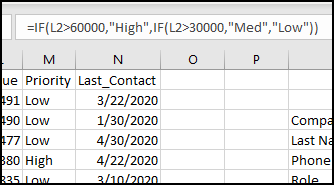
\includegraphics[width=\maxwidth{.75\linewidth}]{gfx/ch09_fig41}
		\caption{IF Formula for M2}
		\label{09:fig41}
	\end{figure}
	
\end{enumerate}

\subsubsection{SumIf/SumIfS}

\[ =SUMIF(range, criteria, [sum\_range]) \]
\[ =SUMIFS(sum\_range, range1, criteria1, [range2], [criteria2], ...) \]

These two functions will calculate a sum but only if certain specified criteria are true. The difference between the two functions is that SUMIF can only have one criterion while SUMIFS can have two or more criteria. Both functions are used in the following exercise.

\begin{enumerate}
	\item This exercise uses the \fmtWorksheet{Contacts} worksheet in the \fmtWorksheet{Contact} workbook.
	\item In cell \fmtLoc{Q19}, enter \fmtTyping{Low Pri Ttl}.
	\item In cell \fmtLoc{Q20}, enter \fmtTyping{Low Pri 2018}.
	\item In cell \fmtLoc{Q21}, enter \fmtTyping{High Pri Ttl}.
	\item In cell \fmtLoc{Q22}, enter \fmtTyping{High Pri 2018}.
	\item In cell \fmtLoc{R19}, enter \fmtTyping{=SUMIF(\$M\$2:\$M\$101, \\"Low", \$L\$2:\$L\$101)}. This formula will find the total value (\fmtLoc{Column L}) for contracts that have \textit{Low} priority (\fmtLoc{Column M}).
	\item In cell \fmtLoc{R20}, enter \fmtTyping{=SUMIFS(\$L\$2:\$L\$101, \\\$M\$2:\$M\$101, "Low", \$K\$2:\$K\$101, 2018)}. This formula will find the total value (\fmtLoc{Column L}) for contracts that have \textit{Low} priority (\fmtLoc{Column M}) and were signed in $ 2018 $ (\fmtLoc{Column K}).
	\item In cell \fmtLoc{R21}, enter \fmtTyping{=SUMIF(\$M\$2:\$M\$101, \\"High", \$L\$2:\$L\$101)}. This formula will find the total value (\fmtLoc{Column L}) for contracts that have \textit{High} priority (\fmtLoc{Column M}).
	\item In cell \fmtLoc{R22}, enter \fmtTyping{=SUMIFS(\$L\$2:\$L\$101, \\\$M\$2:\$M\$101, "High", \$K\$2:\$K\$101, 2018)}. This formula will find the total value (\fmtLoc{Column L}) for contracts that have \textit{High} priority (\fmtLoc{Column M}) and were signed in $ 2018 $ (\fmtLoc{Column K}).
	\item When completed, cell \fmtLoc{R19} should contain $ 616037 $.
	\item When completed, cell \fmtLoc{R20} should contain $ 56504 $.
	\item When completed, cell \fmtLoc{R21} should contain $ 2364510 $.
	\item When completed, cell \fmtLoc{R22} should contain $ 149989 $.
	
	\begin{figure}[H]
		\centering
		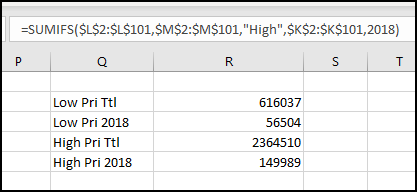
\includegraphics[width=\maxwidth{.75\linewidth}]{gfx/ch09_fig42}
		\caption{SUMIF Formula for R23}
		\label{09:fig42}
	\end{figure}
	
	\item Save the \fmtWorksheet{CH9-Contact} workbook.
	
\end{enumerate}

\subsubsection{CountIf/CountIfS}

\[ =COUNTIF(range, criteria) \]
\[ =COUNTIFS(range1, criteria1, [range2], [criteria2], ...) \]

These two functions will count the number of cells that meet specified criteria. The difference between the two functions is that COUNTIF can only have one criterion while COUNTIFS can have two or more criteria. Both functions are used in the following exercise.

\begin{enumerate}
	\item This exercise uses the \fmtWorksheet{Contacts} worksheet in the \fmtWorksheet{Contact} workbook.
	\item In cell \fmtLoc{Q24}, enter \fmtTyping{Low Pri Count}.
	\item In cell \fmtLoc{Q25}, enter \fmtTyping{Low Pri 2018}.
	\item In cell \fmtLoc{Q26}, enter \fmtTyping{High Pri Count}.
	\item In cell \fmtLoc{Q27}, enter \fmtTyping{High Pri 2018}.
	\item In cell \fmtLoc{R24}, enter \fmtTyping{=COUNTIF(\$M\$2:\$M\$101, "Low")}. This formula counts the number of contracts with a \textit{Low} priority (\fmtLoc{Column M}).
	\item In cell \fmtLoc{R25}, enter \fmtTyping{=COUNTIFS(\$M\$2:\$M\$101, \\"Low", \$K\$2:\$K\$101, 2018)}. This formula counts the number of contracts with a \textit{Low} priority (\fmtLoc{Column M}) and were signed in $ 2018 $ (\fmtLoc{Column K}).
	\item In cell \fmtLoc{R26}, enter \fmtTyping{=COUNTIF($M$2:$M$101, "High")}. This formula counts the number of contracts with a \textit{High} priority (\fmtLoc{Column M}).
	\item In cell \fmtLoc{R27}, enter \fmtTyping{=COUNTIFS($M$2:$M$101, \\"High", $K$2:$K$101, 2018)}. This formula will count the number of contracts with a \textit{High} priority (\fmtLoc{Column M}) and were signed in $ 2018 $ (Column K).
	\item When completed, cell \fmtLoc{R24} should contain $ 39 $.
	\item When completed, cell \fmtLoc{R25} should contain $ 3 $.
	\item When completed, cell \fmtLoc{R26} should contain $ 30 $.
	\item When completed, cell \fmtLoc{R27} should contain $ 2 $.
	
	\begin{figure}[H]
		\centering
		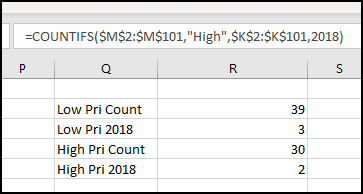
\includegraphics[width=\maxwidth{.75\linewidth}]{gfx/ch09_fig43}
		\caption{COUNTIF Formula for R28}
		\label{09:fig43}
	\end{figure}
		
\end{enumerate}

\subsubsection{Randbetween}

\[ =RANDBETWEEN(bottom, top) \]

It is common to need to generate a random number between two other numbers, like a random number between $ 1 $ and $ 10 $, and the RANDBETWEEN function makes that easy. For this exercise, assume that each of the companies in the data set need to be randomly assigned to one of  three groups for an advertising campaign. The easiest way to do that is to assign a random number between one and three to each of the companies.

\begin{enumerate}
	\item This exercise uses the \fmtWorksheet{Contacts} worksheet in the \fmtWorksheet{Contact} workbook.
	\item In cell \fmtLoc{O1}, enter \fmtTyping{Campaign}.
	\item Adjust the width of \fmtLoc{Column O} to properly display cell \fmtLoc{O1}.
	\item In cell \fmtLoc{O2}, enter \fmtTyping{=RANDBETWEEN(1,3)}. This formula will enter a random number between one and three, inclusive, into cell \fmtLoc{O2}.
	\item Copy cell \fmtLoc{O2} to \fmtLoc{O2:O101}. This will fill \fmtLoc{Column O} with random numbers between one and three.
	\item Note, in Figure \ref{09:fig44}, the numbers in cells \fmtLoc{O2}, \fmtLoc{O3}, and \fmtLoc{O4} were randomly assigned so the student's work may display different values in those cells.
	
	\begin{figure}[H]
		\centering
		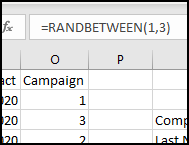
\includegraphics[width=\maxwidth{.50\linewidth}]{gfx/ch09_fig44}
		\caption{RANDBETWEEN Formula for O2}
		\label{09:fig44}
	\end{figure}
	
\end{enumerate}
	
One problem with the RANDBETWEEN function is that new random numbers will be generated whenever any cell on the worksheet is changed. This makes it impossible to come back to the column of random numbers later and expect to find the same values. Follow these steps to correct that shortcoming.

\begin{enumerate}[resume]
	\item Select and copy \fmtLoc{O2:O101}.
	\item Paste Values to \fmtLoc{O2:O101}. Note: it is important to paste the values, not just a simple paste. Otherwise, \fmtLoc{O2:O101} will be filled with the \textit{RANDBETWEEN} formula rather than the value generated by that formula. Note: the values are being saved into the same cells that were used to generate the values. This is a common way used to strip a formula from a cell.
	\item Save the \fmtWorksheet{CH9-Contact} workbook.
\end{enumerate}

\subsubsection{Today/Now}

\[ =TODAY() \]
\[ =NOW() \]

These two functions insert the current date into a worksheet cell. These functions must include the final parenthesis, even if they are empty. The only difference between the two functions is that TODAY inserts only the date while NOW inserts the date and time. Note: the format for the date and time is determined by settings on the computer. These functions are mostly used in the header or footer in print settings.

\begin{enumerate}
	\item This exercise uses the \fmtWorksheet{Contacts} worksheet in the \fmtWorksheet{Contact} workbook.
	\item Insert a new column to the left of \fmtLoc{Column P}. The newly inserted column becomes \fmtLoc{Column P}.
	\item In cell \fmtLoc{P1}, enter \fmtTyping{Contact\_Days} (notice the underscore in the entry).
	\item Adjust the width of \fmtLoc{Column P} to properly display cell \fmtLoc{P1}.
	\item In cell \fmtLoc{P2}, enter \fmtTyping{=VALUE(TODAY()-N2)}. This will subtract the last contact date from today's date to determine how many days have passed since the last contact. Note: Excel will automatically format cell \fmtLoc{P2} as a date since \textit{TODAY()} is in the formula, but \textit{VALUE} makes Excel display the number of days instead of a date.
	\item Copy \fmtLoc{P2} to \fmtLoc{P3:P101}. Note, Figure \ref{09:fig45} shows the number of days as of the date the image was captured, so the student's work will have a different number of days.
	
	\begin{figure}[H]
		\centering
		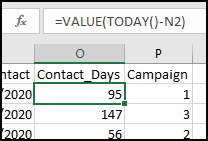
\includegraphics[width=\maxwidth{.50\linewidth}]{gfx/ch09_fig45}
		\caption{Using the Today() Function}
		\label{09:fig45}
	\end{figure}
	
\end{enumerate}

\subsubsection{Date/DateDif}

\[ =DATE(year, month, day) \]
\[ =DATEDIF (start_date, end_date, unit) \]

Excel stores dates as exceptionally large numbers and then calculates the displayed date as the number of days since January $ 1 $, $ 1900 $. For example, January $ 1 $, $ 2020 $ is stored in Excel as $ 43831 $. 

The DATE function converts a date in human-readable form to the number that Excel uses. Thus, \fmtTyping{DATE(2020,01,01)} will be converted to $ 43831 $.

The DATEDIF function calculates the difference in two dates. According to the Microsoft website, ``Excel provides the DATEDIF function to support older workbooks from Lotus $ 1 $-$ 2 $-$ 3 $.'' For some reason, since Excel $ 2000 $, there has been no help in the Excel system for DATEDIF, but the function still works without any problems. 

The \textit{Unit} parameter in the DATEDIF function determines if the difference in two dates is calculated in years (\textit{Y}), months (\textit{M}), or days (\textit{D}).

\begin{enumerate}
	\item This exercise uses the \fmtWorksheet{Contacts} worksheet in the \fmtWorksheet{Contact} workbook.
	\item Insert a new column to the left of \fmtLoc{Column J}. The newly inserted column becomes \fmtLoc{Column J}.
	\item By default, Excel formats cells in an inserted column like the cells in the column to the left of the new column. Therefore, cell \fmtLoc{J2} is formatted as a date since \fmtLoc{I2} is a date. This is normally appropriate, but for this exercise, every cell in \fmtLoc{Column J} needs to be formatted as \textit{General} rather than dates. Select \fmtLoc{Column J} and then click \fmtButton{Home $ \Rightarrow $ Number $ \Rightarrow $ Drop-Down Arrow $ \Rightarrow $ General} to force all cells in the entire column to display using the \textit{General} format.
	\item In cell \fmtLoc{J1}, enter \fmtTyping{Age}.
	\item In cell \fmtLoc{J2}, enter \fmtTyping{=DATEDIF(I2,TODAY(),''Y'')}. This will calculate the number of years between the \textit{birthday} and today's date. 
	\item Copy \fmtLoc{J2} to \fmtLoc{J3:J101}. Note, Figure \ref{09:fig46} shows the age as of the date the image was captured, but student work may have a different age.
	
	\begin{figure}[H]
		\centering
		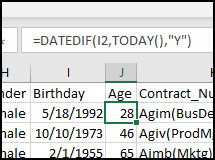
\includegraphics[width=\maxwidth{.50\linewidth}]{gfx/ch09_fig46}
		\caption{Using the Datediff() Function}
		\label{09:fig46}
	\end{figure}
	
	\item It is appropriate to leave the formula in this column instead of removing it as was done for other columns in this exercise. That way, when the workbook is opened in the future, the values in the \textit{Age} column will be automatically updated.
	\item Adjust the width of \fmtLoc{Column J} so all data is properly displayed.
\end{enumerate}

\subsubsection{AND/OR}

\[ =AND(logical1, [logical2], ...) \]
\[ =OR(logical1, [logical2], ...) \]

These two related functions test different logical conditions and return either \textit{TRUE} or \textit{FALSE} depending on the outcome of the test. 

\begin{enumerate}
	\item This exercise uses the \fmtWorksheet{Contacts} worksheet in the \fmtWorksheet{Contact} workbook.
	\item Insert a new column to the left of \fmtLoc{Column K}. The newly inserted column becomes \fmtLoc{Column K}.
	\item In cell \fmtLoc{K1}, enter \fmtTyping{Sales}.
	\item In cell \fmtLoc{K2}, enter \fmtTyping{=AND(G2 = "Sales", J2 \textless 40)}. This will output \textit{TRUE} if \fmtLoc{G2} contains \textit{Sales} and \fmtLoc{J2} is less than $ 40 $. 
	\item Adjust the width of \fmtLoc{Column K} to properly display the value in \fmtLoc{K2}.
	\item Copy \fmtLoc{K2} to \fmtLoc{K3:K101}.
	
	\begin{figure}[H]
		\centering
		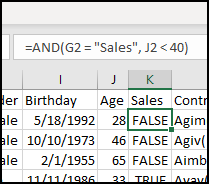
\includegraphics[width=\maxwidth{.75\linewidth}]{gfx/ch09_fig47}
		\caption{Using the AND Function}
		\label{09:fig47}
	\end{figure}

	\item Normally, \textit{AND} and \textit{OR} functions are combined with an \textit{IF} function to make the result more readable.
	\item Change the formula in \fmtLoc{K2} to this: \fmtTyping{=IF(AND(G2 = "Sales", J2 \textless 40),"Yes","")}. This will print \textit{Yes} for lines where the Role (\fmtLoc{Column F})is \textit{Sales} and \textit{Age} (\fmtLoc{Column J}) is less than $ 40 $ but print nothing otherwise. 
	\item Copy \fmtLoc{K2} to \fmtLoc{K3:K101}. Now most cells in \fmtLoc{Column K} will be blank but a few will contain \textit{Yes} where the contact is in the sales department and the age is less than $ 40 $.
\end{enumerate}

\subsubsection{NOT}

\[ =NOT(logical) \]

This function will test different a logical condition and return either \textit{TRUE} or \textit{FALSE} depending on the outcome of the test.

\begin{enumerate}
	\item This exercise uses the \fmtWorksheet{Contacts} worksheet in the \fmtWorksheet{Contact} workbook.
	\item Insert a new column to the left of \fmtLoc{Column E}. The newly inserted column becomes \fmtLoc{Column E}.
	\item In cell \fmtLoc{E1}, enter \fmtTyping{Common}.
	\item In cell \fmtLoc{E2}, enter \fmtTyping{=NOT(D2="Dr")}. This will output \textit{TRUE} if \fmtLoc{E2} contains anything other than \textit{Dr}. 
	\item Copy \fmtLoc{E2} to \fmtLoc{E3:E101}.
	
	\begin{figure}[H]
		\centering
		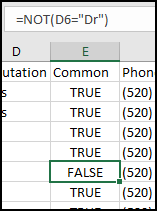
\includegraphics[width=\maxwidth{.50\linewidth}]{gfx/ch09_fig48}
		\caption{Using the NOT Function}
		\label{09:fig48}
	\end{figure}
	
	\item Change \fmtLoc{E2} to: \fmtTyping{=AND(NOT(D2="Dr"), NOT(D2="Rev"))}. This formula uses AND to look for Salutations (\fmtLoc{Column D}) that are not \textit{Dr} AND not \textit{Rev}.
	\item As one final improvement in the formula, change \fmtLoc{E2} to  \\\fmtTyping{=IF(AND(NOT(D2="Dr"), NOT(D2="Rev")), "Yes", "")}. This will print \textit{Yes} for lines where the Salutation (\fmtLoc{Column D}) is anything other than ``Dr'' and ``Rev'' but print nothing otherwise.	
	\item Copy \fmtLoc{E2} to \fmtLoc{E3:E101}.
	\item Adjust the width of \fmtLoc{Column E} so all data is properly displayed.
	\item Save and close the \fmtWorksheet{CH9-Contact} workbook.
\end{enumerate}

%\subsection{Examples}
%
%Here is an example that combine both text and number functions.
%
%	\item Extract information for the oldest person in the list
%	\item See \url{https://exceljet.net/formula/get-information-corresponding-to-max-value}

\begin{center}
	\begin{tkwbox}{Key Take-Aways}
		\textbf{Useful Functions}
		\\
		\begin{itemize}
			\setlength{\itemsep}{0pt}
			\setlength{\parskip}{0pt}
			\setlength{\parsep}{0pt}
			
			\item Excel includes hundreds of functions for both text and numbers, but some are more generally useful than others.  
			\item Excel's most useful text functions include To Columns, Trim, Concatenate, Upper/Lower/Proper, Left/Right/Mid, VLookup, and Index Match.
			\item Excel's most useful number functions include Sum, Average, Min/Max, Round, If, SumIf, CountIf, RandBetween, Today/Now, Date/DateDif, AND/OR, and NOT.
			
		\end{itemize}
	\end{tkwbox}
\end{center}

\section{Statistics}

\begin{center}
	\begin{objbox}{Learning Objectives}
		\begin{itemize}
			\setlength{\itemsep}{0pt}
			\setlength{\parskip}{0pt}
			\setlength{\parsep}{0pt}
			
			\item Use Correlation, Descriptives, and Histogram from the Data Analysis pack.
			
		\end{itemize}
	\end{objbox}
\end{center}

Excel includes an \textit{Analysis Toolpak} that contains $ 19 $ advanced statistics and engineering functions, but it is considered an Add-in and must be activated before it can be used. Most Excel users will never need these types of statistics analysis tools, but they are available if needed.

\begin{enumerate}
	\item Click \fmtButton{File $ \Rightarrow $ Options}.
\end{enumerate}

\begin{figure}[H]
	\centering
	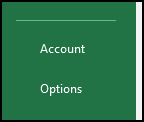
\includegraphics[width=\maxwidth{.50\linewidth}]{gfx/ch09_fig50}
	\caption{The Options Button in the Backstage View}
	\label{09:fig50}
\end{figure}

\begin{enumerate}[resume]	
	
	\item Click \fmtButton{Add-ins} in the left-hand menu of the \textit{Excel Options} pop-up box (see Figure \ref{09:fig51}).
	\item Select \textit{Excel Add-ins} in the drop-down menu at the bottom of the \textit{Add-ins} tab.
	\item Click \fmtButton{Go}.
	
\end{enumerate}

\begin{figure}[H]
	\centering
	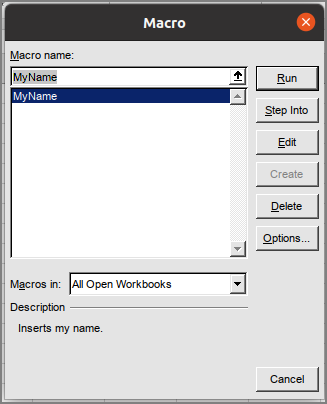
\includegraphics[width=\maxwidth{.95\linewidth}]{gfx/ch09_fig51}
	\caption{The Add-ins Manager}
	\label{09:fig51}
\end{figure}

\begin{enumerate}[resume]	
	
	\item Click the checkbox beside \textit{Analysis Toolpak Add-in} in the \textit{Add-ins} pop-up box. 
	
\end{enumerate}

\begin{figure}[H]
	\centering
	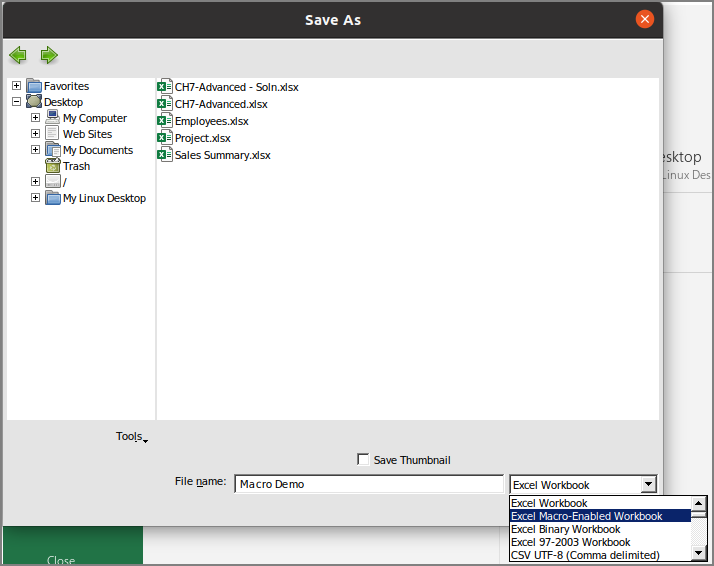
\includegraphics[width=\maxwidth{.75\linewidth}]{gfx/ch09_fig52}
	\caption{Activating The Analysis Toolpak Add-In}
	\label{09:fig52}
\end{figure}

\begin{enumerate}[resume]	
	\item Click \fmtButton{OK}.
\end{enumerate}

Excel adds a new button at \fmtButton{Data $ \Rightarrow $ Analysis $ \Rightarrow $ Data Analysis}.

\begin{figure}[H]
	\centering
	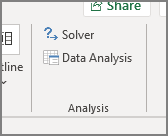
\includegraphics[width=\maxwidth{.50\linewidth}]{gfx/ch09_fig53}
	\caption{The Data Analysis Button}
	\label{09:fig53}
\end{figure}

\begin{enumerate}[resume]	
	\item Open workbook \fmtWorksheet{CH9-Stats.xlsx}.
	\item Save the workbook as \fmtWorksheet{CH9-Cafe}.
	\item This workbook has only one worksheet, \fmtWorksheet{Cafe}.
\end{enumerate}

The Cafe worksheet contains $ 100 $ results of a survey of customers in a small cafe. Note: this is dummy data created for this book.

\subsubsection{Correlation}

A fundamental statistical calculation is the correlation between two variables. A correlation is a number between $ -1.0 $ and $ +1.0 $, where $ 0.0 $ means there is no correlation between the two variables and either $ +1.0 $ or $ -1.0 $ means there is a perfect correlation. A positive correlation means that as one variable increases the other also increases. For example, as people age, they tend to weigh more so a positive correlation would be expected between age and weight. A negative correlation, on the other hand, means that as one variable increases the other decreases. For example, as people age, they tend to run slower so a negative correlation would be expected between age and running speed. For the Cafe data, it would be reasonable to wonder if there is some sort of relationship between the length of the meal and the bill. Longer meals should correlate to higher bills, so a positive correlation would be important for a researcher to know.

\begin{enumerate}[resume]
	\item \fmtOldExcel{Excel 2016} Click \fmtButton{Data $ \Rightarrow $ Analysis $ \Rightarrow $ Data Analysis}. (Note: the statistics functions are identical in Excel $ 2016 $ and Excel $ 365 $, but their group on the ribbon has a slightly different name.)
	\item \fmtNewExcel{Excel 365} Click \fmtButton{Data $ \Rightarrow $ Analyze $ \Rightarrow $ Data Analysis}. (Note: the statistics functions are identical in Excel $ 2016 $ and Excel $ 365 $, but their group on the ribbon has a slightly different name.)
	\item In the \textit{Data Analysis} dialog box, select \textit{Correlation} and click \fmtButton{OK}.
\end{enumerate}

\begin{figure}[H]
	\centering
	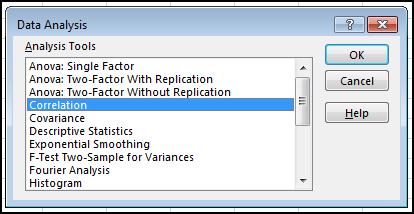
\includegraphics[width=\maxwidth{.95\linewidth}]{gfx/ch09_fig54}
	\caption{Data Analysis Selection Box}
	\label{09:fig54}
\end{figure}

\begin{enumerate}[resume]
	\item The \textit{Correlation} dialog box pops up.
\end{enumerate}

\begin{figure}[H]
	\centering
	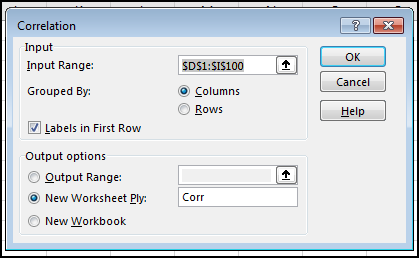
\includegraphics[width=\maxwidth{.75\linewidth}]{gfx/ch09_fig55}
	\caption{Correlation Parameters}
	\label{09:fig55}
\end{figure}

\begin{enumerate}[resume]
	\item Input Range: \fmtTyping{\$D\$1:\$I\$100}
	\item Grouped By: Columns
	\item Labels in First Row: Checked
	\item Output: New Worksheet Ply: \fmtTyping{Corr}
	\item Click \fmtButton{OK}.
	\item Excel creates a new worksheet named \textit{Corr} that contains a correlation table that displays the correlations between the six variables contained in the selected range. Notice that the correlation between \textit{Length} and \textit{Bill} is $ 0.611327 $, which is strong. However, also note that the correlation between \textit{PtySize} (the number in the group) and \textit{Bill} is $ 0.866466 $, which is much stronger. It would stand to reason that a larger group of diners would generate a higher bill.
\end{enumerate}

\begin{figure}[H]
	\centering
	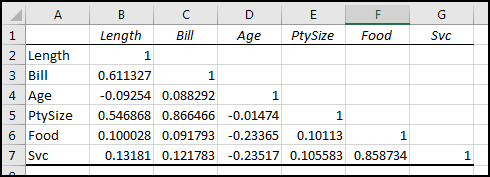
\includegraphics[width=\maxwidth{.95\linewidth}]{gfx/ch09_fig56}
	\caption{Correlation Table}
	\label{09:fig56}
\end{figure}

\subsubsection{Descriptives}

Descriptive statistics summarize a variable with multiple useful calculations. Follow these steps to generate descriptives for \textit{Age}.

\begin{enumerate}[resume]
	\item Click the \fmtWorksheet{Cafe} worksheet to open it.
	\item Click \fmtButton{Data $ \Rightarrow $ Analysis $ \Rightarrow $ Data Analysis}.
	\item In the \textit{Data Analysis} dialog box, select \textit{Descriptive Statistics} and click \fmtButton{OK}.
	\item The \textit{Descriptive Statistics} dialog box pops up.
\end{enumerate}

\begin{figure}[H]
	\centering
	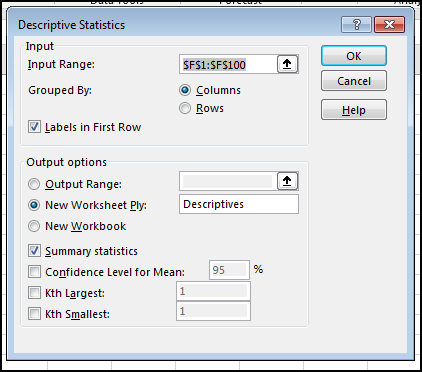
\includegraphics[width=\maxwidth{.75\linewidth}]{gfx/ch09_fig60}
	\caption{Descriptive Statistics Parameters}
	\label{09:fig60}
\end{figure}

\begin{enumerate}[resume]
	\item Input Range: \fmtTyping{\$F\$1:\$F\$100}
	\item Grouped By: Columns
	\item Labels in First Row: Checked
	\item Output: New Worksheet Ply: \fmtTyping{Descriptives}
	\item Summary Statistics: Checked
	\item Click \fmtButton{OK}.
	\item Excel creates a new worksheet named Descriptives that contains a table that displays various descriptive statistics for \textit{Age}. For example, the mean age is $ 41.47475 $.
\end{enumerate}

\begin{figure}[H]
	\centering
	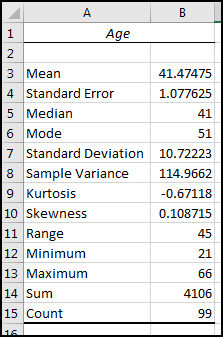
\includegraphics[width=\maxwidth{.50\linewidth}]{gfx/ch09_fig61}
	\caption{Descriptive Statitics}
	\label{09:fig61}
\end{figure}

\subsubsection{Histogram}

A histogram is a graphic representation of a numeric variable. For a histogram, the values are placed in ``bins'' and the number in each bin is counted and graphed. 

\begin{enumerate}[resume]
	\item Click the \fmtWorksheet{Cafe} worksheet to open it.
	\item Click \fmtButton{Data $ \Rightarrow $ Analysis $ \Rightarrow $ Data Analysis}.
	\item In the \textit{Data Analysis} dialog box, select \textit{Histogram} and click \fmtButton{OK}.
	\item The \textit{Histogram} dialog box pops up.
\end{enumerate}

\begin{figure}[H]
	\centering
	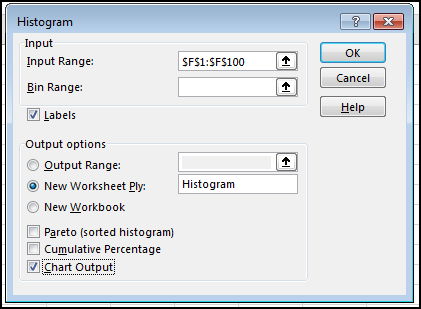
\includegraphics[width=\maxwidth{.75\linewidth}]{gfx/ch09_fig62}
	\caption{Histogram Parameters}
	\label{09:fig62}
\end{figure}

\begin{enumerate}[resume]
	\item Input Range: \fmtTyping{\$F\$1:\$F\$100}
	\item Bin Range: leave blank
	\item Labels: Checked
	\item Output: New Worksheet Ply: \fmtTyping{Histogram}
	\item Chart Output: Checked
	\item Click \fmtButton{OK}.
	\item Excel creates a new worksheet named Histogram that contains a table that displays the counts for each age ``bin.'' For example, $ 15 $ people were between the ages of $ 36 $ and $ 40 $ (inclusive). Also, the histogram graph is displayed for a quick view of how the age data is distributed.
	\item Save and close the \fmtWorksheet{CH9-Cafe} workbook.
\end{enumerate}

\begin{figure}[H]
	\centering
	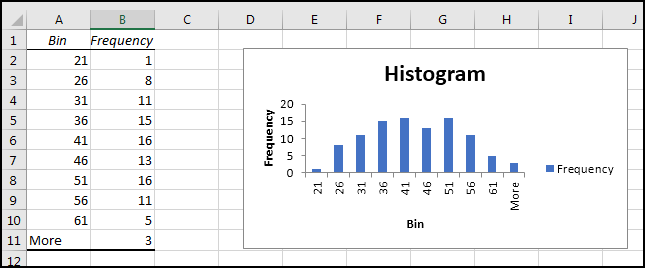
\includegraphics[width=\maxwidth{.95\linewidth}]{gfx/ch09_fig63}
	\caption{Histogram of Age}
	\label{09:fig63}
\end{figure}

\begin{center}
	\begin{tkwbox}{Key Take-Aways}
		\textbf{Statistics}
		\\
		\begin{itemize}
			\setlength{\itemsep}{0pt}
			\setlength{\parskip}{0pt}
			\setlength{\parsep}{0pt}
			
			\item A correlation numerically describes the relationship between two variables.
			\item Descriptives create numerous statistics for a variable.
			\item A histogram graphically represents the distribution for a numeric variable.
			
		\end{itemize}
	\end{tkwbox}
\end{center}

\section{Macros}

\begin{center}
	\begin{objbox}{Learning Objectives}
		\begin{itemize}
			\setlength{\itemsep}{0pt}
			\setlength{\parskip}{0pt}
			\setlength{\parsep}{0pt}
			
			\item Automate simple tasks with a macro.
			
		\end{itemize}
	\end{objbox}
\end{center}

\textit{View $ \Rightarrow $ Macros $ \Rightarrow $ Macros} allows users to automate repetitive tasks. The top part of the button will open the \textit{View Macros} dialog box and the bottom half reveals options for macros. 

\begin{enumerate}
	\item Open a new blank workbook. (\textit{Note}: the macro is placed in a new workbook, so it does not accidentally interfere with the exercises in any other workbook.)
	\item Click \fmtLoc{A1} to select that cell.
	\item Click \fmtButton{View $ \Rightarrow $ Macros $ \Rightarrow $ Macros} (be sure to click the small arrow at the bottom of the \fmtButton{Macros} button).
	\item Select \fmtButton{Use Relative References}.
	\item In the same popup, select \fmtButton{Record Macro}.
	\item Name the macro \fmtTyping{MyName} (note, macro names cannot contain spaces).
	\item Click in the \textit{Shortcut Key} box and type \fmtKeystroke{Q} (this is a capital Q). 
	\item Store the macro in this workbook.
	\item Enter this description: \fmtTyping{Inserts my name}.
\end{enumerate}

\begin{figure}[H]
	\centering
	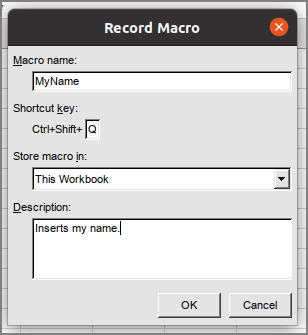
\includegraphics[width=\maxwidth{.75\linewidth}]{gfx/ch09_fig65}
	\caption{The Record Macro Settings Box}
	\label{09:fig65}
\end{figure}

\begin{enumerate}[resume]	
	\item Click \fmtButton{OK}.
	\item Type your first and last name and press \fmtKeystroke{Enter}.
	\item Click \fmtButton{View $ \Rightarrow $ Macros $ \Rightarrow $ Macros} (be sure to click the small arrow at the bottom of the \fmtButton{Macros} button).
	\item Click \fmtButton{Stop Recording}.
\end{enumerate}

Select another cell on the worksheet and press \fmtKeystroke{Ctrl} $ + $ \fmtKeystroke{Shift} $ + $ \fmtKeystroke{Q}. Remember that relative references were activated for the macro, otherwise the name would have always been created in cell \textit{A1} (the original cell) instead of the current cell.

\begin{enumerate}
	\item Click \fmtButton{View $ \Rightarrow $ Macros $ \Rightarrow $ Macros} (be sure to click the top of the \fmtButton{Macros} button).
	\item This opens the \textit{Macro Manager} dialog box where macros can be edited, deleted, or have various options set.
\end{enumerate}

\begin{figure}[H]
	\centering
	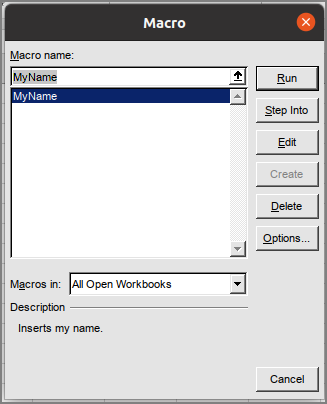
\includegraphics[width=\maxwidth{.75\linewidth}]{gfx/ch09_fig66}
	\caption{The Macro Manager Box}
	\label{09:fig66}
\end{figure}

\begin{enumerate}[resume]	
	\item Click \fmtButton{Cancel} to close the Macro manager.
\end{enumerate}

Remember that all workbooks containing macros must be saved using the ``macro-enabled'' option (that creates a file extension of \textit{.xlsm}). Figure \ref{09:fig67} shows a drop-down menu at the bottom right corner of the \textit{Save-As} screen where \textit{Excel Macro-Enabled Workbook} must be selected. 

\begin{figure}[H]
	\centering
	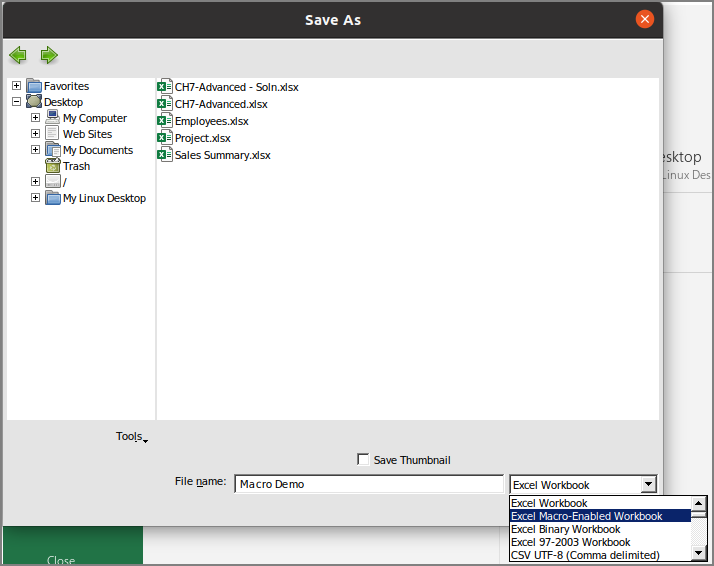
\includegraphics[width=\maxwidth{.95\linewidth}]{gfx/ch09_fig67}
	\caption{Saving a Workbook With a Macro}
	\label{09:fig67}
\end{figure}

Since this macro will not be reused in the future, close the workbook without saving.

\begin{center}
	\begin{tkwbox}{Key Take-Aways}
		\textbf{Using Excel Macros}
		\\
		\begin{itemize}
			\setlength{\itemsep}{0pt}
			\setlength{\parskip}{0pt}
			\setlength{\parsep}{0pt}
			
			\item Macros automate simple tasks to save time in data entry.
			\item Workbooks containing macros must be saved with the ``Macro-Enabled'' setting.
			
		\end{itemize}
	\end{tkwbox}
\end{center}

\section{Excel Preferences}

\begin{center}
	\begin{objbox}{Learning Objectives}
		\begin{itemize}
			\setlength{\itemsep}{0pt}
			\setlength{\parskip}{0pt}
			\setlength{\parsep}{0pt}
			
			\item Explore and optionally change Excel preferences.
			
		\end{itemize}
	\end{objbox}
\end{center}

Like all Microsoft Office products, Excel has scores of preferences and this section lists those that are most adjusted by users.

To find the preferences, click \textit{File $ \Rightarrow $ Options}.

\begin{figure}[H]
	\centering
	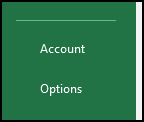
\includegraphics[width=\maxwidth{.95\linewidth}]{gfx/ch09_fig50}
	\caption{The Backstage Options Button}
	\label{09:fig68}
\end{figure}
 
The Options area is divided into $ 11 $ different tabs and each tab includes settings for many preferences. Here is a brief overview of the different option tabs.

\begin{table}[H]
	\rowcolors{1}{}{tablerow} % zebra striping background
	{\small
		%\fontsize{8}{10} \selectfont %Replace small for special font size
		\begin{longtable}{L{1.00in}L{3.00in}} %Left-aligned, Max width: 4.25in
			\textbf{Category} & \textbf{Settings} \endhead
			\hline
			General & These are the commonly modified settings, such as the interface, user name, and Start screen.\\
			Formulas & Settings to control calculations, error-checking, and formulas.\\
			Proofing & Options for spell-check and auto-correct.\\
			Save & Settings that govern saving, autorecovery, and web server options.\\
			Language & Chose the primary and other languages used for editing, tooltips, and help.\\
			Ease of Access & Settings that concern accessibility, including an accessibility checker and various settings for sounds and font.\\
			Advanced & Numerous settings that are not often changed, divided into five areas.\\
			Customize Ribbon & Add and remove items from the ribbon, also rearrange or rename the ribbon tabs and groups.\\
			Quick Access Toolbar & Add and remove items from the Quick Access Toolbar, rearrange the toolbar, and specify its location.\\
			Add-ins & Activate or remove various add-ins.\\
			Trust Center & Manage certificates and other Excel security features.\\
			\rowcolor{captionwhite}
			\caption{Summary of Excel Options}
			\label{09:tab03}
		\end{longtable}
	} % End small
\end{table}

It is not the intent of this book to describe every possible preference but following is a list of those that users commonly modify.

\subsection{General}

\begin{description}
	\item[Enable Live Preview] When changing visual items, like fonts or colors, this previews the change live in the current sheet. This can get annoying, so some users turn it off.
	\item[Screen Tip style] Screen tips are the pop-up boxes with brief help for the various buttons on the ribbon. Some users find these distracting and the can be turned off with this setting.
	\item[Use this as the default font] Use this to change the default font used in new workbooks. Also, the default font size can be set if a larger size is needed.
	\item[Include this many sheets] New workbooks include three blank worksheets by default, but that number can be changed here. Often, one worksheet is enough for new workbooks and then other worksheets can added as needed.
	\item[User name] This is the author's name that is saved with the workbook.
	\item[Show the Start screen when this application starts] Uncheck this box to turn off the start screen.
	\item[Collapse the ribbon automatically] Checking this box will automatically collapse the ribbon into a menu to save space on the screen. The ribbon will drop down when any of the menu items are clicked. It is also easy to pin the ribbon open while working.
\end{description}

\subsection{Formulas}

\begin{description}
	\item[Reset Ignored Errors] Sometimes users have Excel ignore errors as they are developing a worksheet. This button will reset the ignored errors, so all errors are again displayed.
\end{description}

\subsection{Proofing}

This tab includes the various settings for spell-check, like ignore uppercase words. It also includes the Autocorrect options. Normally, the default settings for these items is adequate but that can be changed at this tab.

\subsection{Save}

\begin{description}
	\item[Save AutoRecover information every] Set how often Excel autosaves a workbook. The default is $ 10 $ minutes, but that can be decreased if desired.
	\item[Default local file location] This is the default location for files on initial save or a ``Save As'' operation.
\end{description}

\subsection{Language}

Excel uses the Windows system language and that is normally acceptable. However, this tab makes it possible to change the default Office language for both viewing and editing.

\subsection{Ease of Access}

This tab makes several accessibility options available. 

\subsection{Advanced}
	
	\begin{description}
		\item[After pressing Enter, move selection] By default, Excel moves the selector (active cell) down when the enter key is pressed, but some users prefer the selector to move right and that can be set here.
		\item[Show this number of Recent Workbooks] When Excel opens, it displays the file names for recently opened workbooks. Use this preference to set the number of recent workbooks to display. The default (and maximum number) is $ 50 $.
		\item[Ruler units] Most Americans are comfortable using inches on the ruler, but Excel can also use metric units. The unit used is set with this preference.
		\item[At startup, open all files in] Specify a folder on the hard drive and any Excel files in that folder will be automatically opened when Excel starts. This is a great timesaver while working on a project for several weeks where the same Excel files need to be opened.
	\end{description}
	
\subsection{Customize Ribbon}

The ribbon is highly customizable from this tab. Users can add/remove items from the ribbon, change the order of the items on the ribbon, create new groups, rename items, and generally whatever they want to do to make the ribbon work best for themselves. Customizations can even be exported in a file that can be imported on another computer so users can make Excel on all the computers they use look the same.

In addition to the customizations on this tab, the General Tab includes an option to collapse the ribbon automatically.

\subsection{Quick Access Toolbar}

The Quick Access Toolbar is one of the most useful Excel feature. Users can add links to their most often used Excel functions, so they are easily available without clicking on any ribbon links. The Quick Access Toolbar is set up with the links the user wants. Optionally, the Quick Access Toolbar can be moved to under the ribbon.

The \textit{Quick Access Toolbar} is found at the upper left side of the Excel screen above the Ribbon, as shown in Figure \ref{09:fig68}. This area provides access to the most frequently used commands, such as \textit{Save} and \textit{Undo}. The \textit{Quick Access Toolbar} can be customized by activating commands that are extensively used or inactivating commands that are not needed. By placing these commands in the \textit{Quick Access Toolbar}, it is not necessary to navigate through the Ribbon to find them. To customize the \textit{Quick Access Toolbar}, click the down arrow as shown in Figure \ref{09:fig68}. This will open a menu of commonly used commands that can be added to the \textit{Quick Access Toolbar} by checking them. If the desired command is not on the list, select the \textit{More Commands} option, which opens a screen containing every command on the ribbon. As an additional modification, the \textit{Quick Access Toolbar} and be placed below the ribbon by clicking \textit{Show Below the Ribbon} and many users prefer it in that location.

\begin{figure}[H]
	\centering
	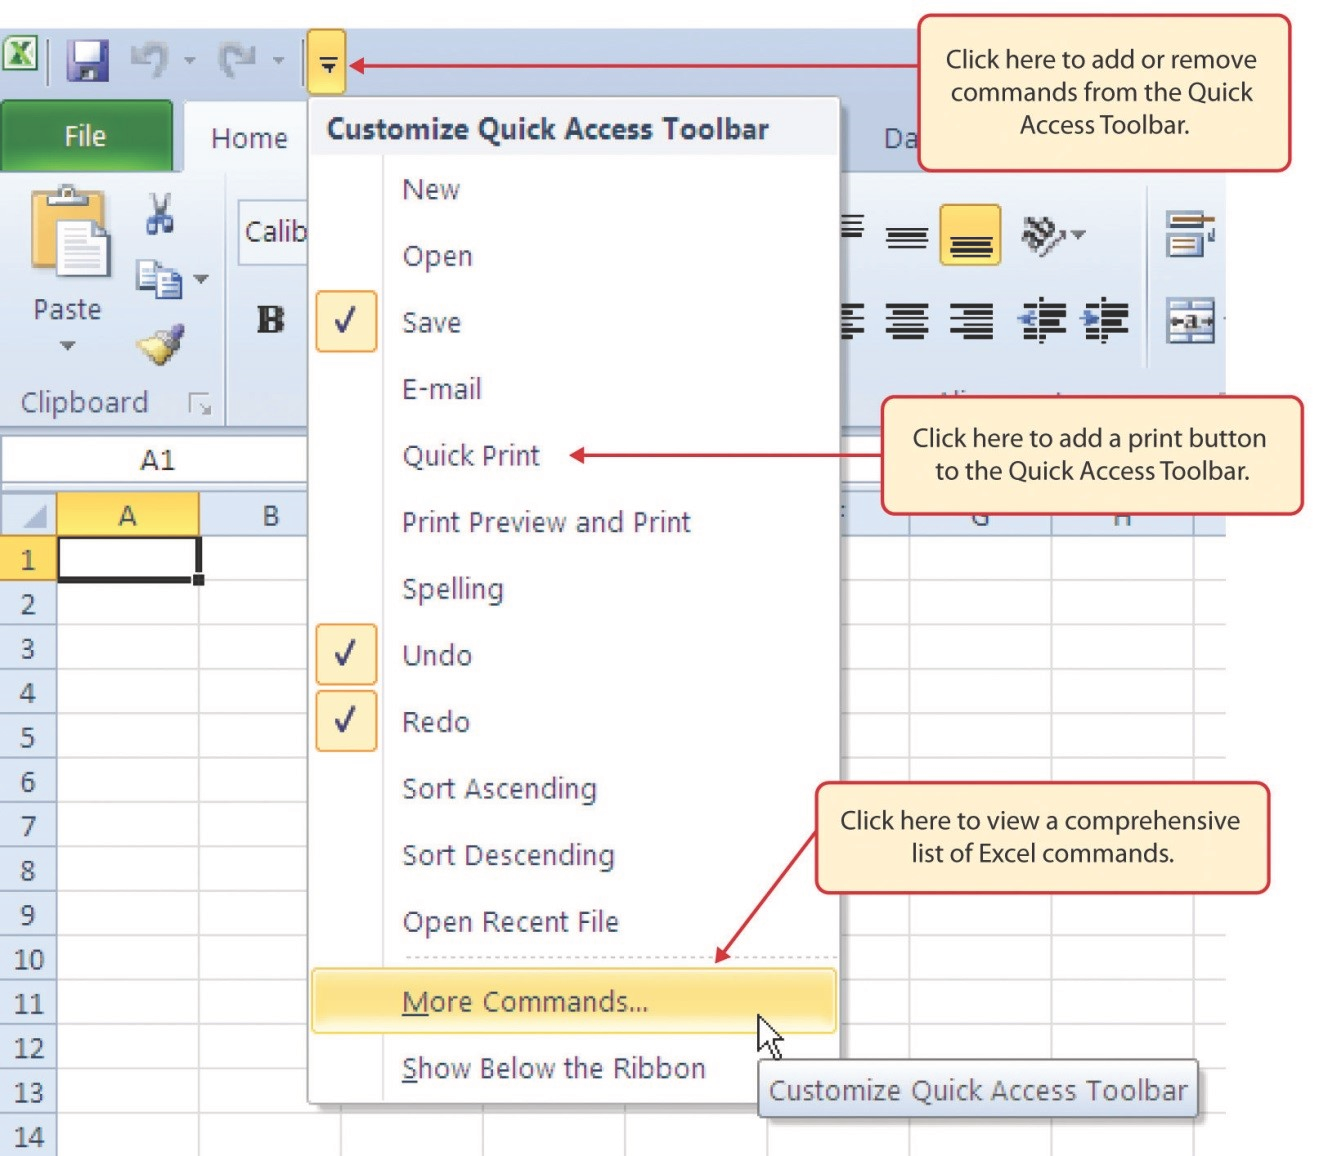
\includegraphics[width=\maxwidth{.75\linewidth}]{gfx/ch09_fig68}
	\caption{Modifying the Quick Access Toolbar}
	\label{09:fig68}
\end{figure}

\subsection{Add-ins}

Any add-ins present in Excel can be activated/deactivated from this tab.

\subsection{Trust Center}

Users can check security certificates or other security settings on this tab.

\begin{center}
	\begin{tkwbox}{Key Take-Aways}
		\textbf{Preferences}
		\\
		\begin{itemize}
			\setlength{\itemsep}{0pt}
			\setlength{\parskip}{0pt}
			\setlength{\parsep}{0pt}
			
			\item Excel includes scores of options that users can change according to their individual preferences.
			
		\end{itemize}
	\end{tkwbox}
\end{center}

\section{Just For Fun}

Excel has had a long and expansive lifetime. It should not be surprising that along the way people who use Excel would find interesting things to do with Excel that are not exactly in the users' manual. This final section of the book lists a few of the fun facts about Excel along with the things people have done with this versatile application.

\subsection{Interesting Bug}

Excel started as a competitive product for Lotus 123. Unfortunately, Lotus 123 counted the year $ 1900 $ as a leap year, though it was not. When Excel was first created, Microsoft decided to use the same serial numbering convention for storing dates so the two programs were compatible; but that meant the year $ 1900 $ was also listed as a leap year in Excel. While this would have been a very easy bug to correct, that would mean that every date after Feb $ 29 $, $ 1900 $ would have been one day off. For this reason, Microsoft decided to leave that leap day in the program. Consequently, to this day, Feb $ 29 $, $ 1900 $ exists in Excel even though there was never a Feb $ 29 $, $ 1900 $ on the calendar. (Reference: \url{https://www.datarails.com/6-cool-facts-excel/})

\subsection{Renaming Genes}

Some genes had to be renamed since Excel automatically formatted the original names as dates. For example, there is a gene that was originally named MARCH1 (for Membrane Associated Ring-CH-Type Finger 1), but whenever MARCH1 is entered in Excel it is formatted as a date. As a result, the HUGO Gene Nomenclature Committee changed the name of this gene to MARCHF1. 27 other genes with the same problem were renamed. (Reference: \url{https://www.engadget.com/scientists-rename-genes-due-to-excel-151748790.html})

\subsection{Art with Excel}

Tatsuo Horiuchi, a 73-year-old Japanese artist, creates some of the most impressive still life art using only Excel as his canvas. Examples of his work, along with a brief explanation of how he creates them, can be found at \url{https://www.demilked.com/73-year-old-excel-paintings-tatsuo-horiuchi/}. 

\begin{figure}[H]
	\centering
	
\includegraphics[width=\maxwidth{.75\linewidth}]{gfx/ch09_fig69}
	\caption{Mr. Horiuchi's Art}
	\label{09:fig69}
\end{figure}

\subsection{Excel and Sudoku}

For fans of \textit{Sudoku}, Peter Mladek created an Excel workbook with macros that can create endless \textit{Sudoku} puzzles. While loading Excel workbooks containing macros found on the web can be risky, this workbook has been around since $ 2004 $ and been used by countless thousands of people; so it would be reasonable to trust it. The free version builds a puzzle and optionally fills the cells with possible solutions. Registering the workbook for \$ $ 9.99 $ opens advanced features that include a solution aid and puzzle creator. Sudoku fans should check out \url{http://www.sudoku-xls.com/} for more information.

\section{Chapter Practice}

\subsection{Cars Analysis}

This exercise uses data on $ 392 $ car models that was collected by David Donoho and Ernesto Ramos for the $ 1982 $ \textit{Exposition of Statistical Graphics Technology} hosted by the \textit{Committee on Statistical Graphics of the American Statistical Association (ASA)}. The dataset is commonly used in statistics classes and can be found at several online locations, including \url{https://github.com/sandialabs/slycat-data}.

\begin{enumerate}
	\item Start Excel and open a new blank workbook.
	\item Save the workbook as \fmtWorksheet{PR9-Cars}.

	\item \fmtOldExcel{Excel 2016} Load the data.
	\begin{enumerate}		
		\item Click \fmtButton{Data $ \Rightarrow $ Get External Data $ \Rightarrow $ From Text}.
		\item Navigate to \fmtWorksheet{PR9-Data.csv}.
		\item Click the file name and then \fmtButton{Import}.
		\item Work through the import wizard.
		\begin{enumerate}
			\item The data in the CSV file has headers.
			\item The data uses a comma delimiter.
			\item Import the data into a new worksheet.
		\end{enumerate}
		\item Click cell \fmtLoc{A1} then click \fmtButton{Insert $ \Rightarrow $ Tables $ \Rightarrow $ Table}.
		\item The \textit{Create Table} dialog box has the correct defaults, so click \fmtButton{OK}.
		\item Click \fmtButton{Yes} on the dialog box with the warning about overlapping ``external data ranges'' to complete the data import.
	\end{enumerate}

	\item \fmtNewExcel{Excel 365} Load the data.
	\begin{enumerate}
		\item Click \fmtButton{Data $ \Rightarrow $ Get \& Transform Data $ \Rightarrow $ From Text/CSV}.
		\item Navigate to \fmtWorksheet{PR9-Data.csv}.
		\item Click the file name and then \fmtButton{Import}.
		\item Excel correctly identifies the data fields in the file, so click \fmtButton{Load} to import the data into a table in a new worksheet.	
	\end{enumerate}		
		
	\item Delete \fmtWorksheet{Sheet1}.
	\item Rename \fmtWorksheet{Sheet2} to \fmtWorksheet{Cars}.
	\item Click \fmtLoc{A1} to activate the table.
	\item In \fmtButton{Table Design $ \Rightarrow $ Properties $ \Rightarrow $ Table Name}, enter \fmtTyping{Cars}.
\end{enumerate}

\begin{enumerate}[resume]

	\item Even though the data loads properly, there are a few adjustments that need to be made. First, the \fmtLoc{Origin} column only lists three different locations by number, but these should be changed to their text equivalent for easier analysis.
	
	\begin{enumerate}
		\item Click the down-arrow on the right side of the \textit{Origin} column header for \fmtLoc{Column I}.
		\item Uncheck all items except \fmtButton{$ 1 $} and then click \fmtButton{OK}.

		\begin{figure}[H]
			\centering
			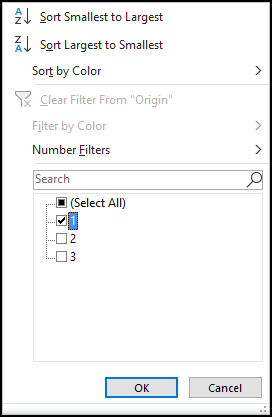
\includegraphics[width=\maxwidth{.65\linewidth}]{gfx/ch09_fig70}
			\caption{Filtering for Location $ 1 $}
			\label{09:fig70}
		\end{figure}

		\item All rows that do not contain a $ 1 $ for \textit{Origin} are hidden. 
		\item Enter \fmtTyping{American} in \fmtLoc{I3} (the cell at the top of the column after rows have been hidden).
		\item Copy/paste \fmtLoc{I3} to all other visible cells in \fmtLoc{Column I}.	Note: using the autofill handle makes this task easier.
		
		\item Click the filter symbol on the right side of the \textit{Origin} column header for \fmtLoc{Column I}.
		\item Uncheck all items except \fmtButton{$ 2 $} and then click \fmtButton{OK}.
		\item All rows that do not contain a $ 2 $ for \textit{Origin} are hidden. 
		\item Enter \fmtTyping{European} in \fmtLoc{I2} (the cell at the top of the column after rows have been hidden).
		\item Copy/paste \fmtLoc{I2} to all other visible cells in \fmtLoc{Column I}.	Note: using the autofill handle makes this task easier.

		\item Click the filter symbol on the right side of the \textit{Origin} column header for \fmtLoc{Column I}.
		\item Uncheck all items except \fmtButton{$ 3 $} and then click \fmtButton{OK}.
		\item All rows that do not contain a $ 3 $ for \textit{Origin} are hidden. 
		\item Enter \fmtTyping{Japanese} in \fmtLoc{I4} (the cell at the top of the column after rows have been hidden).
		\item Copy/paste \fmtLoc{I4} to all other visible cells in \fmtLoc{Column I}.	Note: using the autofill handle makes this task easier.
		
		\item Click the filter symbol on the right side of the \textit{Origin} column header for \fmtLoc{Column I}.
		\item Check \fmtButton{(Select All)} then \fmtButton{OK} to reveal all rows in the data set.
		\item Adjust the width of \fmtLoc{Column I} to fit the data.
		\item Save the \fmtWorksheet{PR9-Cars} workbook.

	\end{enumerate}

	\item Next, data in the \fmtLoc{Model} column needs to be split out so the automobile make and model are separated.
	
	\begin{enumerate}
		\item Insert a column to the left of \fmtLoc{Column B}. The new column becomes \fmtLoc{Column B} with a header of \textit{Column1}.
		\item Enter this formula in \fmtLoc{B2}: \fmtTyping{=PROPER(LEFT(A2,FIND(" ",A2)-1))}. If Excel does not paste that formula to the bottom of the table, then copy/paste it to \fmtLoc{B3:B393}. Excel extracts the make of the car, which is the first word in \fmtLoc{Column A}.
		\item Adjust the width of \fmtLoc{Column B} to fit the data.
		\item Insert a column to the left of \fmtLoc{Column C}. The new column becomes \fmtLoc{Column C} with a header of \textit{Column2}.
		\item Copy \fmtLoc{B2:B393}.
		\item Paste Values to \fmtLoc{C2}. Note: it is important to paste the values, not just a simple paste. Otherwise, \fmtLoc{Column C} will be filled with the formula rather than the value generated by that formula.
		\item Delete \fmtLoc{Column B}.

		\item Insert a column to the left of \fmtLoc{Column C}. The new column becomes \fmtLoc{Column C} with a header of \textit{Column3}.
		\item Enter this formula in \fmtLoc{C2}: \fmtTyping{=PROPER(RIGHT(A2,LEN(A2)-FIND(" ",A2)))}. If Excel does not paste that formula to the bottom of the table, then copy/paste it to \fmtLoc{C3:C393}. Excel extracts the model of the car, which is everything except the first word in \fmtLoc{Column A}.
		\item Insert a column to the left of \fmtLoc{Column D}. The new column becomes \fmtLoc{Column D} with a header of \textit{Column4}.
		\item Copy \fmtLoc{C2:C393}.
		\item Paste Values to \fmtLoc{D1}. Note: it is important to paste the values, not just a simple paste. Otherwise, \fmtLoc{Column D} will be filled with the formula rather than the value generated by that formula.
		\item Delete \fmtLoc{Column C}.
		\item At this point, the data in \fmtLoc{Column A} should be split between \fmtLoc{Column B} and \fmtLoc{Column C}.
		\item Delete \fmtLoc{Column A}.
		\item Enter \fmtTyping{Make} in \fmtLoc{A1}.
		\item Enter \fmtTyping{Model} in \fmtLoc{B1}.

	\end{enumerate}

	\item Click the filter symbol on the right side of the \textit{Make} column header for \fmtLoc{Column A}.
	\item Select \fmtButton{Sort A to Z}.
	\item Adjust the width of \fmtLoc{Column A} and \fmtLoc{Column B} to fit the data.
	
	\item The data preparation is complete so save the \fmtWorksheet{PR9-Cars} workbook.

\end{enumerate}

Once a data table is prepared it can be used for analysis. For this exercise, several different analysis techniques are used.


\begin{enumerate}
	\item Create a new worksheet and name it \fmtTyping{Summary}.
	\item Move \fmtWorksheet{Summary} to the left of \fmtWorksheet{Cars} so it is the first worksheet in the workbook.
	\item Click the \fmtWorksheet{Summary} tab to activate that sheet.
	\item Select \fmtLoc{A1:G1} and click \fmtButton{Home $ \Rightarrow $ Alignment $ \Rightarrow $ Merge \& Center}.
	\item In cell \fmtLoc{A1}, enter \fmtTyping{Automobile Statistics}.
	\item Format cell \fmtLoc{A1}.
	
	\begin{itemize}
		\item Calibri font, 18 pt
		\item Bold style
		\item Font color: Orange, Accent 2, Darker 25\%
	\end{itemize}
	
	\item In cell \fmtLoc{E3}, enter \fmtTyping{Cylinders}.
	\item In cell \fmtLoc{E4}, enter \fmtTyping{4}.
	\item In cell \fmtLoc{F3}, enter \fmtTyping{Year}.
	\item In cell \fmtLoc{F4}, enter \fmtTyping{71}.
	
	\item In cell \fmtLoc{B3}, enter \fmtTyping{Max MPG, Cyl 4, Yr 71}.
	\item Adjust the width of \fmtLoc{Column B} to fit the text in \fmtLoc{B3}.
	\item In cell \fmtLoc{C3}, enter \fmtTyping{=DMAX(Cars[\#All], ''MPG'', \$E\$3:\$F\$4)}.
	\item Excel reports $ 35 $ as the maximum MPG for $ 1971 $ cars with $ 4 $ cylinders.
	
	\begin{figure}[H]
		\centering
		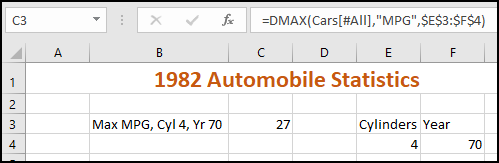
\includegraphics[width=\maxwidth{.95\linewidth}]{gfx/ch09_fig71}
		\caption{Calculating the Max MPG}
		\label{09:fig71}
	\end{figure}
	
	\item In cell \fmtLoc{B4}, enter \fmtTyping{Avr MPG, Cyl 4, Yr 71}.
	\item In cell \fmtLoc{C4}, enter \fmtTyping{=DAVERAGE(Cars[\#All], ''MPG'', \$E\$3:\$F\$4)}.
	\item Excel reports $ 25.66667 $ as the average MPG for $ 1970 $ cars with $ 4 $ cylinders.
	
	\item In cell \fmtLoc{F4}, enter \fmtTyping{$ 72 $}. Notice that Excel automatically updates \fmtLoc{C3} and \fmtLoc{C4} to reflect the values for $ 1972 $ cars.
	\item In cell \fmtLoc{F4}, enter \fmtTyping{$ 71 $} to change back to that year and match the labels in \fmtLoc{B3} and \fmtLoc{B4}.

	\item In cell \fmtLoc{B5}, enter \fmtTyping{Avr MPG, Cyl 4-6, Yr 71}.
	\item In cell \fmtLoc{E5}, enter \fmtTyping{$ 6 $}
	\item In cell \fmtLoc{F5}, enter \fmtTyping{$ 71 $}.
	\item In cell \fmtLoc{C5}, enter \fmtTyping{=DAVERAGE(Cars[\#All], ''MPG'', \$E\$3:\$F\$5)}.
	\item Excel reports $ 23.8 $ as the average MPG for $ 1971 $ cars with $ 4 $ or $ 6 $ cylinders. 
\end{enumerate}	
	
Excel reads the criteria range such that items in a single row are joined with an ``AND'' and multiple rows are joined with an ``OR.'' Thus, the criteria in \textit{E3:F5} reads \textit{(Cars with $ 4 $ cylinders AND year $ 71 $) OR (Cars with $ 6 $ cylinders AND year $ 71 $)}. Complex Boolean conditions can be specified using multiple rows and columns.

If a cell in a criteria range is empty, then Excel matches it to all entries in the data table.

\begin{enumerate}[resume]

	\item Delete the data in \fmtLoc{F5}. Notice that the value in \fmtLoc{C5} changes to $ 20.94526 $. The criteria in this case reads \textit{(Cars with $ 4 $ cylinders AND year $ 70 $) OR (Cars with $ 6 $ cylinders AND all model years}. 
	\item In cell \fmtLoc{F5}, enter \fmtTyping{$ 71 $}.
	\item In cell \fmtLoc{G3}, enter \fmtTyping{Origin}.
	\item In cell \fmtLoc{G4}, enter \fmtTyping{American}.
	\item In cell \fmtLoc{B6}, enter \fmtTyping{Avr MPG, Cyl 6, Yr 71, American}.
	\item Adjust the width of \fmtLoc{Column B} to fit the text in \fmtLoc{B6}.
	\item In cell \fmtLoc{C6}, enter \fmtTyping{=DAVERAGE(Cars[\#All], ''MPG'', \$E\$3:\$G\$4)}.
	\item Excel reports $ 24.75 $ as the average MPG for $ 1971 $ cars with $ 4 $ cylinders made in America. 
	
	\item Complete the summary worksheet using the following information. Adjust the width of \fmtLoc{Column B} as necessary to display the text entered there.
	
\end{enumerate}	

\begin{table}[H]
	\rowcolors{1}{}{tablerow} % zebra striping background
	{\small
		%\fontsize{8}{10} \selectfont %Replace small for special font size
		\begin{longtable}{L{0.5in}L{3.50in}} %Left-aligned, Max width: 4.25in
			\textbf{Cell} & \textbf{Content} \endhead
			\hline
			\fmtLoc{B7} & \fmtTyping{Max MPG, American}\\
			\fmtLoc{C7} & \fmtTyping{=DMAX(Cars[\#All],"MPG",\$G\$3:\$G\$4)}\\

			\fmtLoc{F8} & \fmtTyping{Year}\\
			\fmtLoc{G8} & \fmtTyping{Origin}\\
			\fmtLoc{F9} & \fmtTyping{$ <76 $}\\
			\fmtLoc{G9} & \fmtTyping{American}\\
			\fmtLoc{B8} & \fmtTyping{Min MPG, Yr\textless76, American}\\
			\fmtLoc{C8} & \fmtTyping{=DMIN(Cars[\#All],"MPG",\$F\$8:\$G\$9)}\\

			\fmtLoc{F10} & \fmtTyping{$ <76 $}\\
			\fmtLoc{G10} & \fmtTyping{European}\\
			\fmtLoc{B9} & \fmtTyping{Avr MPG, Yr\textless76, American or European}\\
			\fmtLoc{C9} & \fmtTyping{=DAVERAGE(Cars[\#All],"MPG",\$F\$8:\$G\$10)}\\
			
			\rowcolor{captionwhite}
			\caption{Information To Complete The Summary Table}
			\label{05:tab01}
		\end{longtable}
	} % End small
\end{table}

The Figure \ref{09:fig72} shows the Summary Table at this point, but it could easily be extended with various combinations of criteria to extract whatever information is desired from the cars data. 

\begin{figure}[H]
	\centering
	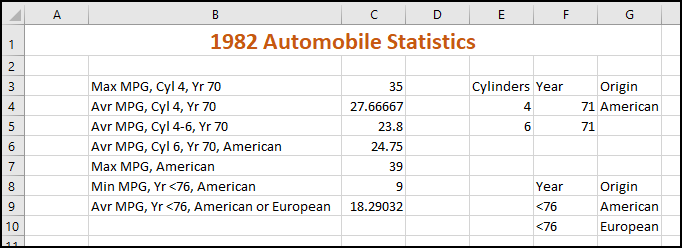
\includegraphics[width=\maxwidth{.95\linewidth}]{gfx/ch09_fig72}
	\caption{Summary Table}
	\label{09:fig72}
\end{figure}


\begin{enumerate}[resume]

	\item Save the \fmtWorksheet{PR9-Cars} workbook.
	\item Click in \fmtLoc{B12} to activate that cell.
	\item Click \fmtButton{Data $ \Rightarrow $ Analyze $ \Rightarrow $ Data Analysis}.
	\item Select \fmtButton{Correlation} in the \textit{Data Analysis} dialog box, then click \fmtButton{OK}.
	
	\begin{figure}[H]
		\centering
		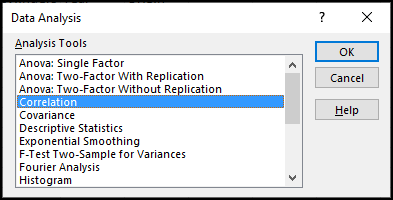
\includegraphics[width=\maxwidth{.95\linewidth}]{gfx/ch09_fig73}
		\caption{Data Analysis Popup}
		\label{09:fig73}
	\end{figure}
	
	\item Enter the following in the \textit{Correlation} dialog box.
	
	\begin{itemize}
		\item \textbf{Input Range}: \fmtTyping{'Cars'!\$C\$1:\$H\$393}
		\item \textbf{Grouped By}: Columns
		\item \textbf{Labels in first row}: Checked
		\item \textbf{Output Range}: \$B\$12
	\end{itemize}

	\begin{figure}[H]
		\centering
		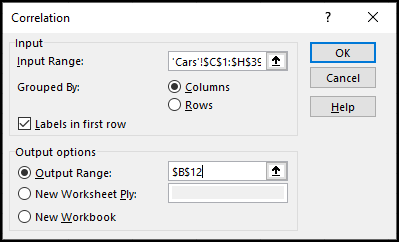
\includegraphics[width=\maxwidth{.75\linewidth}]{gfx/ch09_fig74}
		\caption{Correlation Parameters}
		\label{09:fig74}
	\end{figure}
	
	\item Click \fmtButton{OK}.
	\item Adjust the column widths so all information in \fmtLoc{Row 12} is visible.
	\item Excel calculates the various correlations and displays them in \fmtLoc{B12:H18}. There are several rather extreme correlations in the table, but all would be expected. For example, the correlation between weight and MPG is $ -0.83224 $, so heavier cars get fewer miles per gallon.
	
	\begin{figure}[H]
		\centering
		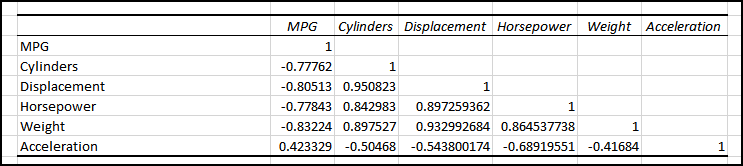
\includegraphics[width=\maxwidth{.95\linewidth}]{gfx/ch09_fig75}
		\caption{Correlation Results}
		\label{09:fig75}
	\end{figure}

	\item Click in \fmtLoc{B21} to activate that cell.
	\item Click \fmtButton{Data $ \Rightarrow $ Analyze $ \Rightarrow $ Data Analysis}.
	\item Select \fmtButton{Histogram} in the \textit{Data Analysis} dialog box, then click \fmtButton{OK}.
	\item Enter the following in the \textit{Histogram} dialog box.

	\begin{itemize}
		\item \textbf{Input Range}: \fmtTyping{'Cars'!\$C\$1:\$C\$393}
		\item \textbf{Labels}: Checked
		\item \textbf{Output Range}: \$B\$21
		\item \textbf{Chart Output}: Checked
	\end{itemize}
	
	\begin{figure}[H]
		\centering
		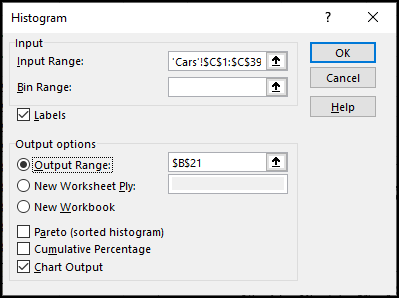
\includegraphics[width=\maxwidth{.75\linewidth}]{gfx/ch09_fig76}
		\caption{Histogram Parameters}
		\label{09:fig76}
	\end{figure}

	\item Click \fmtButton{OK}.
	\item Excel displays the histogram data and chart. 
	\item Adjust the chart so the top left corner is in \fmtLoc{D22} and the bottom right corner is in \fmtLoc{K38}.
	\item Using the \textit{Chart Elements} selector, remove the legend from the histogram.
	\item Change the title of the histogram to \fmtTyping{Automobile MPG}.
	\item Change the X\textit{-Axis} title to \fmtTyping{MPG}.

	\begin{figure}[H]
		\centering
		\includegraphics[width=\maxwidth{.95\linewidth}]{gfx/ch09_fig77}
		\caption{Histogram Results}
		\label{09:fig77}
	\end{figure}
	
	\item Save and close the \fmtWorksheet{PR9-Cars} workbook. Submit the workbook to the instructor as directed.

\end{enumerate}


\section{Scored Assessment}

\subsection{Weather Analysis}

The \textit{National Oceanic and Atmospheric Administration (NOAA)} makes all their weather data available for researchers to investigate.\footnote{The data for this exercise was downloaded and adapted from \url{https://www.ncdc.noaa.gov/cdo-web/}.}

\begin{enumerate}
	\item Open workbook \fmtWorksheet{SC9-Data}.
	\item Save the workbook as \fmtWorksheet{SC9-Climate}.
\end{enumerate}

This workbook has two worksheets. The \fmtWorksheet{Data} sheet contains the raw data that will be analyzed for this exercise and the \fmtWorksheet{Notes} sheet contains definitions for the abbreviations used on the \fmtWorksheet{Data} sheet.

\begin{enumerate}[resume]
	\item Calculate the number of hours of daylight for each day.
	
	\begin{enumerate}
		\item Insert a new column to the left of \fmtLoc{Column N}.
		\item In cell \fmtLoc{N1}, enter \fmtTyping{Daylight}.
		\item In cell \fmtLoc{N2}, enter \fmtTyping{=M2-L2}.
		\item Copy/paste \fmtLoc{N2} to \fmtLoc{N3:N363}.
		\item Click \fmtButton{Home $ \Rightarrow $ Number $ \Rightarrow $ Down Arrow $ \Rightarrow $ More Number Formats}. 
		\item In the \textit{Format Cells} dialog box, select \fmtButton{Time} in the \textit{Category} list and then select \fmtButton{37:30:55} in the \textit{Type} list. This will format the data in \fmtLoc{Column N} to the number of hours/minutes elapsed between sunrise and sunset.
		
		\begin{figure}[H]
			\centering
			\includegraphics[width=\maxwidth{.75\linewidth}]{gfx/ch09_fig80}
			\caption{Formatting The Daylight Column}
			\label{09:fig80}
		\end{figure}
		
		
	\end{enumerate}
	
	\item Use the following steps to convert the data to a table.
	
	\begin{enumerate}
		\item Click in \fmtLoc{A1} to activate that cell.
		\item Click \fmtButton{Insert $ \Rightarrow $ Tables $ \Rightarrow $ Table}.
		\item Excel will automatically select the entire data set, \fmtLoc{\$A\$1:\$O\$363}. Be sure \fmtButton{My table has headers} is checked.
		\item Click \fmtButton{OK}.
		\item Name the table \fmtTyping{Climate}.
	\end{enumerate}
	
	\begin{figure}[H]
		\centering
		\includegraphics[width=\maxwidth{.75\linewidth}]{gfx/ch09_fig85}
		\caption{Climate Table Name}
		\label{09:fig85}
	\end{figure}
	
	\item Create a new worksheet and name it \fmtTyping{Summary}.
	\item Move \fmtWorksheet{Summary} to the left of \fmtWorksheet{Data} so it is the first worksheet in the workbook.
	\item Click the \fmtWorksheet{Summary} tab to activate that sheet.
	\item Select \fmtLoc{A1:G1} and click \fmtButton{Merge \& Center}.
	\item In cell \fmtLoc{A1}, enter \fmtTyping{2019 Ft Huachuca Climate Information}.
	\item Format cell \fmtLoc{A1}.
	
		\begin{itemize}
			\item Calibri font, 18 pt
			\item Bold style
			\item Font color: Blue, Accent 1
		\end{itemize}

	\item In cell \fmtLoc{B3}, enter \fmtTyping{Date}. (Note: this will be the starting date for formulas on this sheet, but the title in \fmtLoc{B3} must match the field name on the \textit{Climate} table.)
	\item In cell \fmtLoc{C3}, enter \fmtTyping{Date}. (Note: this will be the ending date for formulas on this sheet, but the title in \fmtLoc{C3} must match the field name on the \textit{Climate} table.)
	\item In cell \fmtLoc{B4}, enter \fmtTyping{$ >=1/1/2019 $} (Note: do not leave spaces in this formula).
	\item In cell \fmtLoc{C4}, enter \fmtTyping{$ <=1/31/2019 $} (Note: do not leave spaces in this formula).
	\item In cell \fmtLoc{B5}, enter \fmtTyping{Max Temp}.
	\item Adjust the width of \fmtLoc{Column B} and \fmtLoc{Column C} so everything is visible.
	\item In cell \fmtLoc{C5}, enter this formula: \fmtTyping{=DMAX(Climate[\#All], ''TMAX'', \$B\$3:\$C\$4)}.
	\item Cell \fmtLoc{C5} will display $ 72 $, which is the greatest \textit{TMAX} for January, $ 2019 $.

	\begin{figure}[H]
		\centering
		\includegraphics[width=\maxwidth{.95\linewidth}]{gfx/ch09_fig86}
		\caption{Maximum January Temperature}
		\label{09:fig86}
	\end{figure}

	\item Change the dates to \fmtTyping{$ >=3/1/2019 $} and \fmtTyping{$ <=3/31/2019 $} to find that the maximum March temperature is $ 82 $.
	\item Change the dates back to \fmtTyping{$ >=1/1/2019 $} and \fmtTyping{$ <=1/31/2019 $} to complete the other activities on the summary sheet.

	\item In cell \fmtLoc{B6}, enter \fmtTyping{Min Temp}.
	\item In cell \fmtLoc{C6}, enter this formula: \fmtTyping{=DMIN(Climate[\#All], ''TMIN'', \$B\$3:\$C\$4)}.
	\item Cell \fmtLoc{C6} will display $ 21 $, which is the least \textit{TMIN} for January, $ 2019 $.

	\item In cell \fmtLoc{B7}, enter \fmtTyping{Precipitation}.  (The width of \fmtLoc{Column B} may need to be changed to see the word \textit{Precipitation}.)
	\item In cell \fmtLoc{C7}, enter this formula: \fmtTyping{=DSUM(Climate[\#All], ''PRCP'', \$B\$3:\$C\$4)}.
	\item Cell \fmtLoc{C7} will display $ 0.9 $, which is the total precipitation for January, $ 2019 $.

	\item In cell \fmtLoc{B8}, enter \fmtTyping{Wind Speed}.
	\item In cell \fmtLoc{C8}, enter this formula: \fmtTyping{=DAVERAGE(Climate[\#All], ''AWND'', \$B\$3:\$C\$4)}.
	\item Cell \fmtLoc{C8} will display $ 8.002258065 $, which is the average wind speed for January, $ 2019 $.
	\item To make \fmtLoc{C8} easier to read, click \fmtButton{Home $ \Rightarrow $ Number $ \Rightarrow $ Decrease Decimal} to reduce \fmtLoc{C8} to two decimal places, $ 8.00 $.

	\item In cell \fmtLoc{B9}, enter \fmtTyping{Max Wind}.
	\item In cell \fmtLoc{C9}, enter this formula: \fmtTyping{=DMAX(Climate[\#All], ''WSF5'', \$B\$3:\$C\$4)}.
	\item Cell \fmtLoc{C9} will display $ 42.90 $, which is the greatest wind gust for January, $ 2019 $.

	\item Copy/paste \fmtLoc{B3:C4} to \fmtLoc{B11:C12}.
	\item In cell \fmtLoc{D11}, enter \fmtTyping{Moon}.
	\item In cell \fmtLoc{D12}, enter \fmtTyping{New}.
	\item In cell \fmtLoc{C12}, enter \fmtTyping{$ <= 12/31/2019 $}.
	\item In cell \fmtLoc{B13}, enter \fmtTyping{Coldest New Moon}. (The width of \fmtLoc{Column B} may need to be changed to see the words \textit{Coldest New Moon}.)
	\item In cell \fmtLoc{C13}, enter this formula: \fmtTyping{=DMIN(Climate[\#All], ''TMIN'', \$B\$11:\$D\$12)}.
	\item Cell \fmtLoc{C13} will display $ 32 $, which was the coldest temperature recorded on a night with a new moon in $ 2019 $.

	\item Copy/paste \fmtLoc{B11:D12} to \fmtLoc{B15:D16}.
	\item In cell \fmtLoc{D15}, enter \fmtTyping{DailyWeather} (Note: there is no space between the two words).
	\item In cell \fmtLoc{D16}, enter \fmtTyping{*TS*}. Note: the asterisks are ``wildcard'' characters and will create a match on any cell that contains \textit{TS} somewhere in the cell.
	\item In cell \fmtLoc{B17}, enter \fmtTyping{Largest Storm}.
	\item In cell \fmtLoc{C17}, enter this formula: \fmtTyping{=DMAX(Climate[\#All], ''PRCP'', \$B\$15:\$D\$16)}.
	\item Cell \fmtLoc{C17} will display $ 2.32 $, which was the most rainfall on a day that recorded thunder in $ 2019 $.
	
	\begin{figure}[H]
		\centering
		\includegraphics[width=\maxwidth{.95\linewidth}]{gfx/ch09_fig87}
		\caption{Various Summary Statistics}
		\label{09:fig87}
	\end{figure}

	\item Save the \fmtWorksheet{SC9-Climate} workbook.
	
\end{enumerate}	

Next, create a chart that shows the amount of daylight throughout the year. (Note: the process for creating charts is covered in more detail in Chapter \ref{ch04:charts}, page \pageref{ch04:charts}.)

\begin{enumerate}
	\item Click the \fmtWorksheet{Data} worksheet to activate it.
	\item Click the top of \fmtLoc{Column N} to activate that column.
	\item Click \fmtButton{Insert $ \Rightarrow $ Charts $ \Rightarrow $ Insert Line or Area Chart}.
	\item In the \textit{Line Chart} dialog box, select the first option, \fmtButton{2-D Line}.
	\item Excel will create a line chart that shows the amount of daylight throughout the year. 
	
	\begin{figure}[H]
		\centering
		\includegraphics[width=\maxwidth{.95\linewidth}]{gfx/ch09_fig88}
		\caption{Daylight Chart: Start}
		\label{09:fig88}
	\end{figure}
	
	\item Right-click the chart and select \fmtButton{Move Chart}. Move it as an object in the \fmtWorksheet{Summary} worksheet.

	\begin{figure}[H]
		\centering
		\includegraphics[width=\maxwidth{.95\linewidth}]{gfx/ch09_fig89}
		\caption{Daylight Chart: Moving to Summary Worksheet}
		\label{09:fig89}
	\end{figure}

	\item Drag/drop the chart so the top-left corner is about at the center of cell \fmtLoc{B20}.
	\item By default, the horizontal axis simply counts the number of entries from $ 1 $ to $ 363 $, but it should display the dates found in \textit{Column A}.
	\item Click the chart area to display the three buttons on the right side of the chart. Click the \fmtButton{Chart Filters} button, which looks like a funnel.
	
	\begin{figure}[H]
		\centering
		\includegraphics[width=\maxwidth{.50\linewidth}]{gfx/ch09_fig90}
		\caption{Daylight Chart: Chart Filters}
		\label{09:fig90}
	\end{figure}

	\item Notice that the \textit{Categories} filter is just a list of numbers, starting at one. Click the \fmtButton{Select Data} button at the bottom right corner of the \textit{Values} dialog box. The \textit{Select Data Source} dialog box appears.

	\begin{figure}[H]
		\centering
		\includegraphics[width=\maxwidth{.75\linewidth}]{gfx/ch09_fig91}
		\caption{Daylight Chart: Select Data Source}
		\label{09:fig91}
	\end{figure}
	
	\item Click \fmtButton{Edit} for the \textit{Horizontal (Category) Axis Labels}. That button is marked in Figure \ref{09:fig91}.
	\item Enter \fmtTyping{=Data!\$A\$2:\$A\$363} for the Axis label range.
	
	\begin{figure}[H]
		\centering
		\includegraphics[width=\maxwidth{.75\linewidth}]{gfx/ch09_fig92}
		\caption{Daylight Chart: Axis Labels}
		\label{09:fig92}
	\end{figure}
	
	\item Excel changes the labels for the \textit{X-Axis} to the dates found in \fmtLoc{Column A} of the \fmtWorksheet{Data} worksheet. Click \fmtButton{OK} on the \textit{Select Data Source} dialog box to finish this selection.
	\item To adjust the scale for the \textit{Y-Axis} (the hours of daylight), right-click on the vertical axis values and select \fmtButton{Format Axis}.
	\item In the \textit{Format Axis} dialog box, enter \fmtTyping{$ 0.35 $} for the \textit{Minimum Bounds} (the \textit{Maximum Bounds} will automatically adjust).
	
	\begin{figure}[H]
		\centering
		\includegraphics[width=\maxwidth{.95\linewidth}]{gfx/ch09_fig93}
		\caption{Daylight Chart: Adjusting Y-Axis Scale}
		\label{09:fig93}
	\end{figure}
	
	\item Save and close the \fmtWorksheet{SC-Climate} workbook. Submit it to the instructor as directed.
\end{enumerate}





	


